\documentclass[final,1p]{elsarticle}
\usepackage{amssymb}
\usepackage{stackrel}
\usepackage{amsfonts}
\usepackage{amsmath}
\usepackage[english]{babel}
\usepackage{graphicx}
\usepackage{float}
\usepackage{rotating}
\usepackage{color}
%\usepackage{ulem}
\usepackage{tikz}
\usepackage{epic}
% \usepackage{caption,subcaption}
%\usepackage{subeqnarray}
 

\newcommand\encircle[1]{%
  \tikz[baseline=(X.base)] 
    \node (X) [draw, shape=circle, inner sep=0] {\strut #1};}

\newcommand{\I}{\mathrm{i}}
\newcommand{\D}{\mathrm{d}}

\newcommand{\PGR}[1]{{\color{blue} #1}}
\newcommand{\PGRcomm}[1]{{\color{blue}\small\em PGR2all: #1}}
\newcommand{\PGRfoot}[1]{{\color{blue}\footnote{\color{blue} #1}}}
%\newcommand{\ES}[1]{{\color{red} #1}}
%\newcommand{\ESfoot}[1]{{\color{red}\footnote{\color{red} #1}}}
\newcommand{\bmu}{{\mbox{\boldmath{$\mu$}}}}

\newcounter{denselistcounter}
\newenvironment{denselist}[1]
{ \begin{list}
  {#1{denselistcounter})}{\usecounter{denselistcounter}
  \setlength{\topsep}{-0pt}
  \setlength{\partopsep}{-0pt}
  \setlength{\itemsep}{-0pt}
  \setlength{\parsep}{-0pt}
  \setlength{\labelwidth}{6pt}
  \setlength{\labelsep}{4pt}
  \setlength{\leftmargin}{20pt}
  \setlength{\rightmargin}{20pt}
  }
}
{\end{list}}

\unitlength 1mm
\thicklines

\begin{document}


\begin{frontmatter}

\title{Documentation for the RTA code in 3D}

\author{F.~Coppens$^a$}
\author{M.~Vincendon$^a$}
\author{P.-G.~Reinhard$^c$}
\author{E.~Suraud$^{a,b}$}
\cortext[author]{Corresponding author:
  coppens@irsamc.ups-tlse.fr} 
\address{$^a$Universit\'e de Toulouse; UPS; Laboratoire de Physique
             Th\'{e}orique, IRSAMC; F-31062 Toulouse Cedex, France}
\address{$^b$Laboratoire de Physique Th\'eorique, Universit\'e Paul
  Sabatier, CNRS, F-31062 Toulouse C\'edex, France}
\address{$^c$Institut f{\"u}r Theoretische Physik, Universit{\"a}t
  Erlangen, D-91058 Erlangen, Germany}

\date{Status: 12. January 2019}
\begin{abstract}
\PGR{\em This is a first draft for the CPC presenting the TDLDA+RTA code
  to the public. The layout of presentation has yet to be discussed.
Presently it mixes theory and algorithm with code. We may also
consider collecting all theory \& numerics together then followed by a
huge block detailing the code.}
\end{abstract}

\begin{keyword}
%\PACS{05.30.Fk,31.70.Hq,34.10.+x,36.40.Cg}
electronic dissipation, time-dependent
density functional theory, ...
\end{keyword}
\end{frontmatter}

\tableofcontents


\section{Introduction}

\PGRcomm{... yet to be written ...}


\noindent
\PGRcomm{Two general points yet to be clarified:
\\
The code is still capable of coupling to a dielectric
  environment. We should skip that for the CPC publication.
\\
Another question to be discussed is whether we maintain the option to
run finite differences instead of FFT. If we do so, then we have to
test that branch carefully.
}


\section{Formal background: electronic DFT coupled to ionic motion}
\label{sec:TDLDA}


\subsection{Brief introduction to TDLDA-MD}

\PGRcomm{The explanation of formal background is extremely compact and
reduced to the basic formula. Here we should provide a brief overview
of the history of DFT and of the physics behind.}

\subsection{The total energy of the model}
\label{sec:Etot}

The basic dynamical variables are the set of single-particle
(s.p.) wavefunctions with their occupation probabilities at the side
of electrons and classical coordinates and momenta for the ions,
together
\begin{equation}
\begin{array}{lcl}
  \mbox{s.p. wavefunctions:} && 
  \varphi_\alpha\;,\;\alpha=1...\Omega
  \quad,
\\
  \mbox{s.p. occupation probabilities:} && 
  w_\alpha\;,\;\alpha=1...\Omega
  \quad,
\\
  \mbox{ionic coordinates:} &&
  \mathbf{R}_I\;,\; I=1,N_\mathrm{ion}
  \quad,
\\
  \mbox{ionic momenta:} &&
  \mathbf{P}_I\;,\; I=1,N_\mathrm{ion}
  \quad.
\end{array}
\end{equation}
A key quantity in connection with energy-density functionals
is the electronic local density 
\begin{equation}
  \varrho_\uparrow\mathbf{r})
  =
  \sum_{\alpha\in\uparrow}w_\alpha
  \varphi_\alpha^+(\mathbf{r})\varphi_\alpha^{\mbox{}}(\mathbf{r})
  \quad,\quad
  \varrho_\downarrow\mathbf{r})
  =
  \sum_{\alpha\in\downarrow}w_\alpha
  \varphi_\alpha^+(\mathbf{r})\varphi_\alpha^{\mbox{}}(\mathbf{r})
  \quad,
\label{eq:locdens}
\end{equation}
which covers, in fact, two separate densities for spin-up and
spin-down. To simplify the presentation of the formalism we
ignore this distinction in the following and use simply
one density $\varrho(\mathbf{r})$.


Starting point is an expression for the total energy of the coupled
electronic and ionic system:
\begin{subequations}
\label{eq:Etotal}
\begin{eqnarray}
  E_\mathrm{total}
  &=&
  E_\mathrm{kin}
  +
  E_\mathrm{C}
  +
  E_\mathrm{xc}
  +
  E_\mathrm{ext}
  +
  E_\mathrm{el,ion}
  +
  E_\mathrm{kin.ion}
  +
  E_\mathrm{pot,ion}
  \;,
\\
  E_\mathrm{kin}[\{\varphi_\alpha\}]
  &=&
  \int d\mathbf{r}\,\sum_\alpha w_\alpha
  \varphi_\alpha^+\frac{\hat{p}^2}{2m}\varphi_\alpha^{\mbox{}}
  \quad,
\label{eq:Ekin}
\\
  E_\mathrm{C}[\varrho]
  &=&
  \frac{e^2}{2}\int d^3rd^3r'\,
  \frac{\varrho(\mathbf{r})\varrho(\mathbf{r}')}{|\mathbf{r}-\mathbf{r}'|}
\\
  E_\mathrm{xc}[\varrho]
  &=&
  \int d\mathbf{r}\,\varrho(\mathbf{r})
  \epsilon_\mathrm{xc}\left(\varrho(\mathbf{r})\right)
  \quad,
\\
  E_\mathrm{ext}[\varrho,t]
  &=&
  \int d\mathbf{r}\,\varrho(\mathbf{r})V_\mathrm{ext}(\mathbf{r},t)
  \quad,
\\
  E_\mathrm{el,ion}[\{\varphi_\alpha\},\{\mathbf{R}_I\}]
  &=&
  \sum_I\int d\mathbf{r}\,\sum_\alpha w_\alpha
  \varphi_\alpha^+
  \hat{V}_\mathrm{PsP}(\mathbf{r}-\mathbf{R}_I)\varphi_\alpha^{\mbox{}}
  \quad,
\\
  E_\mathrm{kin,ion}(\mathbf{P}_I)
  &=&
  \sum_I\frac{\mathbf{P}_I^2}{2M_I}
  \quad,
\\
  E_\mathrm{pot,ion}(\mathbf{R}_I)
  &=&
  \frac{1}{2}\sum_{J\neq I}\frac{e^2}{|\mathbf{R}_I-\mathbf{R}_J|}
  +
  V_\mathrm{ext,ion}(\mathbf{R}_I,t)
  \quad,
\end{eqnarray}
\end{subequations}
where functionals of density are wavefunctions are indicated by square
brackets and functions of coordinates by round brackets.  The
$E_\mathrm{C}$ is the direct part of the electronic Coulomb energy.
The $E_\mathrm{xc}$ is the energy-density functional for electronic
exchange and correlations for which we use in the code two options:
the functional of \cite{Per92} or the older from from \cite{Gun76}.
The $E_\mathrm{ext}$ stands for the excitation mechanisms by external
sources, either from a photon pulse of from the Coulomb field of a
fast bypassing ion, see section \ref{sec:laser}. This part is, of
course, absent in static calculations of the ground state.  The
$E_\mathrm{el,ion}$ carries the interaction with the ions which is
usually described by a pseudo-potential $\hat{V}_\mathrm{PsP}$, see
section \ref{sec:practPsP}, or may be simplified in terms of the
jellium model, see section \ref{sec:jell}.  Ionic kinetic and
potential energy are described by the obvious classical expressions.
The $V_\mathrm{ext,ion}$ in the ionic potential energy describes the
action of an external field on the ions (which is usually negligible
as compared to the effect on the electrons).

\subsubsection{Self-interaction correction (SIC)}
\label{sec:SIC}

\PGRcomm{We have yet to decide which levels of SIC we keep in the code
and then explain them here properly.}

\subsubsection{The pseudo-potentials}
\label{sec:practPsP}

There is a great variety of pseudo-potentials available.  The code
employs two variants. Particularly efficient and simple to use are
local pseudo-potentials integrated from a pseudo-density which is
represented as sum of Gaussians.  The corresponding potential is then
a sum of error functions
\begin{subequations}
\begin{eqnarray}
  V_\mathrm{PsP}(\mathbf{r})
  &=&
  \sum_{i=1}^2 c_i \frac{\mbox{erf}(\mathbf{r}/\sigma_i)}{|(\mathbf{r})|}
  \quad,
\label{eq:locPsP}
\\
  \mbox{erf}(x) 
  &=&
  \sqrt{\frac{2}{\pi}}\int_0^x dy\,e^{-y^2}
  \quad,
\label{eq:erf}
\end{eqnarray}
\end{subequations}
where the $\sigma_i$ are widths and the strength parameters $c_i$ have
to line up to the total charge of the ionic core
$c_1+c_2=Z_\mathrm{ion}$. This pseudo-potential is well suited for
alkaline atoms for which it was originally developed \cite{Kue99}.

More involved, but also more versatile in the applicability, is the
pseudo-potential from \cite{Goe96} which is composed from a local and
a non-local part as
\begin{subequations}
\begin{eqnarray}
  \hat{V}_\mathrm{PsP}
  &=&
  {V}_\mathrm{loc}(\mathbf{r}-\mathbf{R})
  +
  \hat{V}_\mathrm{nloc}
  \quad,
\\
  V_\mathrm{loc}(\mathbf{r}-\mathbf{R})
  &=&
  -\frac{Z_\mathrm{ion}}{x}\mbox{erf}\left(x\right)
  +e^{-x^2}
   \sum_{n=0}^3C_{n+1} 2^{n} x^{2n}
  \quad,\quad
  x
  =
  \frac{|\mathbf{r}-\mathbf{R}|}{r_\mathrm{loc}}
  \quad,
\\
  \hat{V}_\mathrm{nloc}(\mathbf{r},\mathbf{r}')
  &=&
  \sum_{jl\mu}{\cal G}(\mathbf{r}-\mathbf{R}){\cal H}_{jl}{\cal G}(\mathbf{r}'-\mathbf{R})
  \quad,
\label{eq:nonloc}
\end{eqnarray}
where $\mathbf{R}$ is the position of the ionic core with respect to
which the pseudo-potential is defined.  The ${\cal G}$ in the
non-local part (\ref{eq:nonloc} serve to project out the electronic
states which are occupied in the ionic core. These projector functions
for the first few quantum numbers read
\begin{eqnarray}
  {\cal G}_{000}(\mathbf{x})
  &=&
  r_\mathrm{nloc}^{-3}\pi^{-3/2}
  \exp{\left(-\frac{x^2}{2r_\mathrm{nloc}^{2}}\right)}
  \quad,
\\
  {\cal G}_{01\mu}(\mathbf{x})
  &=&
  \sqrt{\frac{2}{3}}r_\mathrm{nloc}\nabla_\mu{\cal G}_{000}(\mathbf{x})
  \quad,
\label{eq:defineGl1}\\
  {\cal G}_{100}(\mathbf{x})
  &=&
  \frac{r_\mathrm{nloc}^{2}}{\sqrt{6}}
  \left(2\Delta-\frac{3}{r_\mathrm{nloc}^{2}}\right)
  {\cal G}_{000}(\mathbf{x})
  \quad.
\end{eqnarray}
\end{subequations}
The projection looks expensive at first glance. However, one can
exploit the fact that the Gaussians cover only a small region space of
order of a few multiples of the non-local radius $r_\mathrm{nloc}$.
Thus one needs to evaluate the projector only on a small sub-grid
which reduces expense dramatically.

\subsubsection{The soft jellium model for the ionic background}
\label{sec:jell}

The electronic wavefunctions of metals and metal clusters are spread
softly over the whole system and hardly resolve the spatial structure
the ionic cores. This allow to replace the detailed ionic background
by a smooth, positive background density. 
Such jellium approximation
is a standard in the theory of bulk metals \cite{Ash76} and the
adaptation to a finite cluster is straightforward. One carves from
bulk jellium a finite element of constant positive charge
corresponding to the average bulk density. The volume is chosen such
that its total charge coincides with the given ionic charge.  For
finite clusters, it is advantageous to use jellium with a soft surface
profile. This is more suited for numerical handling and it improves
the quality of the model, e.g., by producing a correct peak energy for
the optical response of metal clusters \cite{Rub91}. Versatile and
easy to handle in this respect is a Woods-Saxon profile for the
jellium density
\begin{subequations}
\label{eq:softJ}
\begin{eqnarray}
  \varrho_\mathrm{jel}(\mathbf{r})
  &=&
  \frac{3}{4\pi r_s^3}
  \left[1+
     \exp\left(\frac{|\mathbf{r}|-R(\vartheta,\phi)}
                    {\sigma_\mathrm{jel}}\right)
  \right]^{-1}
  \quad,
\\
\noindent \mathrm{with}  \qquad R(\vartheta,\phi)
  &=&
  R_\mathrm{jel}\left(1+\sum_{lm}\alpha_{lm}Y_{lm}(\vartheta,\phi)\right)
  \quad,
\label{eq:defjell}
\\
  \int d\mathbf{r}\, \varrho_\mathrm{jel} 
  &=&
  N_\mathrm{ion}
  \quad.
\label{eq:R0cond}
\end{eqnarray}
\end{subequations}
The jellium radius $R_\mathrm{jel}$ is determined by
eq. (\ref{eq:R0cond}), the normalization to desired number of ions.
The central density is determined by the bulk density
$\rho_0={3}/({4\pi r_s^3})$ and the Wigner-Seitz radius $r_s$ is a
genuine material parameter \cite{Ash76}. The $\sigma_\mathrm{jel}$
parametrizes the surface width and the transition from 90\% to 10\%
bulk density is achieved within $4\sigma_\mathrm{jel}$.  The model does
also allow to describe deformed clusters by angular dependence
$R(\vartheta,\phi)$ of the extension. This is achieved through the
deformation coefficients $\alpha_{lm}$ weighting the impact of the
spherical harmonics. For example, axially symmetric ellipsoids are
tuned by $\alpha_{20}$, positive values producing prolate and negative
values oblate shapes. The $\alpha_{30}$ generate octupole (pear-like)
shapes which have considerable influence in metal cluster spectroscopy
and $\alpha_{40}$ generates hexadecapole which play a role for
fine-tuning the shape \cite{Mon95b}.  Triaxial shapes are produced by
moments with $m\neq 0$. The cluster radius $R_\mathrm{jel}$ is fixed by
the others parameters through eq. (\ref{eq:R0cond}) which is to be
solved numerically by a root finding procedure.  After all, the
leading parameters of the soft jellium model Eq. (\ref{eq:softJ}) are
the Wigner-Seitz radius $r_s$ and the surface thickness $\sigma_{\rm
  jel}$.  They are universal for a given material. Typical values are
$r_s\sim 4\,\mathrm{a}_0$ with $\sigma_\mathrm{jel}\sim
0.9\,\mathrm{a}_0$ for Na clusters, $r_s\sim 2.66\,\mathrm{a}_0$ and
$\sigma_\mathrm{jel}\sim 0.76\,\mathrm{a}_0$ for {Mg clusters}, or
$r_s\sim 3\,\mathrm{a}_0$ and $\sigma_\mathrm{jel}\sim
0.78\,\mathrm{a}_0$ for Ag clusters. The deformation parameters
$\alpha_{lm}$ depend on the actual cluster and strongly vary with
system and size.


The jellium approximation then consists in discarding the ionic
contribution to the total energy (\ref{eq:Etotal}), i.e. the terms
$E_\mathrm{kin,ion}$ and $E_\mathrm{pot,ion}$, and to replace the
pseudo-potential background in $E_\mathrm{el,ion}$ by the Coulomb
potential of the jellium density (\ref{eq:softJ}). There is no
dynamics associated with the jellium. The model thus applies to
situations where ionic motion can be ignored.



\subsubsection{Phenomenological electronic shell models}
\label{eq:phenshell}

Experience shows that KS potentials for metal clusters have a typical
profile characterized by a flat bottom and a smooth transition to
zero. For neutral clusters, one can approximate that very well by a
Woods-Saxon profile
\begin{equation}
  V_\mathrm{WS}(\mathbf{r})
  =
  -V_0
  \left[1+
     \exp\left(\frac{|\mathbf{r}|-R(\vartheta,\phi)}
                    {\sigma_\mathrm{WS}}\right)
  \right]^{-1}
  \quad,
\label{eq:WSpot}
\end{equation}
where, again, a possible deformation can be parametrized by an angular
dependence of the radius
%
$R(\vartheta,\phi)=
R_0\left(1\!+\!\sum_{lm}\alpha_{lm}Y_{lm}(\vartheta,\phi)\right)$,
%
similar to the jellium model of Eq. (\ref{eq:softJ}) for the density.
In Eq. (\ref{eq:WSpot}) the potential depth $V_0$ is taken as the
average binding potential in bulk matter. Computations in a fixed
potential are somewhat simpler than with the self-consistent
scheme. The Woods-Saxon model has thus been very often used for
describing the electronic shell structure of clusters, particularly in
early studies, for a review see \cite{Bra93}. It is meanwhile somewhat
out of fashion. But we provide it in the code for quick tests and
comparison.

A substantial further simplification is achieved by realizing that
shell effects are determined by the states near the Fermi surface and
that these states practically see a harmonic potential. This suggests
to use for first estimates a simple harmonic oscillator shell
model. To mimic surface profile of the Woods-Saxon potential and so
reproduce the sequence of shell closures in metal clusters
 a phenomenologically tuned $\hat{l}^2$ term is added to the
oscillator model.
This yields the Clemenger-Nilsson model for the mean field potential
\begin{equation} 
  \hat{V}_\mathrm{CN}
  =
  \frac{m}{2}\left(
  \omega_x^2x_{\mbox{}}^2+\omega_y^2y_{\mbox{}}^2+\omega_z^2z_{\mbox{}}^2
  \right)
  -
  V_{l2}\hbar\bar{\omega}\left(\hat{l}^2-n(n+3)/6\right)
\label{eq:CleNil}
\end{equation}
where $n$ is the global shell number ($n=n_x+n_y+n_z$). The three
separate curvatures $\omega_i$ allow one to accommodate deformed situations
including triaxiality. Volume conservation restricts their choice to
$\omega_x\omega_y\omega_z=\omega_0^3=$constant. The separate values
can also be expressed in terms of the quadrupole deformation
$\alpha_{lm}$ as introduced above and in Eq. (\ref{eq:softJ}),
e.g. for axially symmetric shapes by
%
$\omega_x=\omega_y=\omega_0\exp{(\alpha_{20}\sqrt{5/4\pi})},
 \omega_z=\omega_0\exp{(-2\alpha_{20}\sqrt{5/4\pi})}$.
%
The parameter $V_{l2}$ serves to tune the downshift of high angular
momentum orbits and thus of the shell sequence.
%
The Clemenger-Nilsson model was introduced into clusters physics in
\cite{Cle85} taking up a much similar nuclear oscillator model
\cite{Nil55}. An extensive review of early applications is given in
\cite{Hee93}. The oscillator model is kept in the code mainly for
testing because one has analytical the solutions for $V_{l2}=0$.

Both shell models, Woods-Saxon or harmonic oscillator, overrule the
total energy (\ref{eq:Etotal}). What remains is only the kinetic
energy (\ref{eq:Ekin}) together with the given model potentials.
Also this approach is, as the jellium model, applicable only in
circumstances where ionic motion plays little role.



\subsubsection{External excitation fields}
\label{sec:laser}


Lasers are the most important and very flexible means for a dedicated,
well tuned excitation of electronic systems.  They produce a strong
coherent electromagnetic field which can be well approximated by a
classical time-dependent electromagnetic field.Typical wavelengths are
in the range of several hundredths of nm. This is a huge distance as
compared to the spatial extension of atoms, molecules, and (most)
clusters.  One can thus treat the laser field in the limit of long
wavelengths ($k \rightarrow 0$) which means to deal with a spatially
homogeneous electrical field $\mathbf{E}$ at the cluster site and we
can neglect the effect of the magnetic field.  The coupling
Hamiltonian leaves of gauge transformation \cite{Jac62}.
The external-field operator in velocity gauge reads\PGRfoot{I am not
  sure that we should show velocity gauge. It may be useful when
  explaining the computation of PES later on.}
\begin{equation}
  V_\mathrm{ext}
  =
  e\mathcal{\mathbf{E}}_0F(t)\hat{\mathbf{p}}
  \quad,\quad
  F(t)
  =
  \int dt'\,f(t')\exp{(-\mathrm{i}\omega_\mathrm{las}t')}
  \quad,
\label{eq:laserp}
\end{equation}
where $f(t')$ is the envelope of the photon pulse.
The same pulse in space gauge becomes
\begin{equation}
  V_\mathrm{ext}
  =
  e{\cal\bf E}_0f(t)\!\cdot\!\hat{\mathbf{r}}
  \exp{(-\mathrm{i}\omega_\mathrm{las}t)}
\label{eq:laserr}
\end{equation}
which is simpler to handle because the laser field acts here simply as
a time-dependent local operator. The code thus uses the external field
in space gauge. Transformation to velocity gauge, if needed, can
be performed a posteriori by standard rules of gauge transformation
\cite{Mes95aB}\PGRfoot{Cross ref to phase correction in PES in section
\ref{sec:observ}.}.
%
The photon pulse is characterized by frequency
$\omega_\mathrm{las}$, peak field strength $E_0=|\mathbf{E}_0|$,
polarization $\mathbf{E}_0/E_0$, and time profile $f(t)$. The
field strength is usually parametrized in terms of the laser intensity
$I$ as
\begin{equation}
  E_0
  =
  c_{EI}
  I^{1/2}
  \quad,\quad
  c_{EI}
  =
  1.07*10^{-8}
  \frac{\mathrm{eV}}{\mathrm{a}_0}
  \left(\frac{\mathrm{W}}{\mathrm{cm}^2}\right)^{-1/2}
  \quad.
\end{equation}
The profile is a matter of debate.  The experimental pulse profiles
are not precisely known either.  It is assumed to be a well peaked
function with a certain full-width at half maximum (FWHM), in practice
well approximated by a Gaussian.  In order to have a finite support
for the pulse, we use the sin$^2$ pulse
\begin{equation}
  f(t)
  =
  \left\{\begin{array}{ll}
    \sin^2{\left(\pi\frac{t}{2T_\mathrm{pulse}}\right)}
        &\mbox{for}\quad t\in\{0,2T_\mathrm{pulse}\}  \\
    0  &\mbox{else}
  \end{array}\right.
  \quad.
\label{eq:sinpulse}
\end{equation}
%\end{subequations}
It is close to a Gaussian pulse in the vicinity of peak field strength
and combines high spectral selectivity with finite bounds. Note that
the form (\ref{eq:sinpulse}) is scaled such that the pulse parameter
$T_\mathrm{pulse}$ is identical with the {full-width at
half-maximum} ({FWHM}).


%\subsubsection{Charged projectiles}

Probing electronic systems by beams of charged particles is a standard
tool in atomic and molecular physics \cite{Bra92} and is also used in
cluster physics. Highly charged ions, protons and to some extend also
electrons can be considered as being structureless. What counts is
only their Coulomb field.  Charged ions are heavy and can be treated
with classical trajectories
%
$\mathrm{R}_\mathrm{ext}(t)$.
%
For sufficiently heavy and fast projectiles, one can approximate
these trajectories by straight lines and that is what is done in the
code.  In any case, the effect of the ion (charge $Z_\mathrm{ext}$) on
the system can again be described by a time dependent external field
\begin{equation}
  V_\mathrm{ext}(\mathbf{r},t)
  =
  \frac{Z_\mathrm{ext}e^2}{|\mathbf{r}-\mathbf{R}_\mathrm{ext}(t)|}
  \quad.
\label{eq:ionext}
\end{equation}
Magnetic effects are neglected. They may play a role only for extremely
fast ions in the relativistic domain.
%
The ionic trajectories are characterized by the ion velocity
$v_\mathrm{ion}$ and the impact parameter $b_\mathrm{ion}$ which is
the distance of closest approach. The velocity is more or less well
defined by the experimental setup. But the impinging ion beam will
cover a broad range of impact parameters. From the theoretical side,
one has then to run several calculations with systematically varied
impact parameters.  Reaction cross sections are then computed by
integration of the reaction probability over impact parameters, for
examples see \cite{Rei98a}.


\subsection{Equations of motion}
\label{sec:mf}

\subsubsection{Electronic Kohn-Sham equations}

Static and dynamical equations determining structure and dynamics of
the electron cloud are determined by variation of the total energy
with respect to the s.p. wavefunctions $\varphi_\alpha$.  This yields
what is called the Kohn-Sham (KS) equations \cite{Koh65}.  We use
energy-density functionals \cite{Per92,Gun76} i.e. functionals in
local density approximation (LDA).  The dynamical application is
called time-dependent LDA (TDLDA) and we use this acronym also in
cases where we add SIC (see section \ref{sec:SIC}) to the treatment.

The time-dependent KS equations determining the propagation of
electronic ground wavefunctions are
\begin{subequations}
\label{eq:KS}
\begin{eqnarray}
  \hat{h}_{\mathrm{KS}}\varphi_\alpha
  &=&
  \mathrm{i}\partial_t\varphi_\alpha
  \quad\mbox{for}\quad
  \alpha\in\{1,...,N_\mathrm{el}\}
  \quad,
\label{eq:TDKS}
\\
  \hat{h}_{\mathrm{KS}}
  &=&
  \frac{\hat{p}^2}{2m}
  +
  \underbrace{
    V_\mathrm{C}(\mathbf{r})
    +
    \hat{V}_{\mathrm{xc}}
    +
    \hat{V}_\mathrm{back}
    +
    V_\mathrm{ext}(\mathbf{r},t)
  }_{V_\mathrm{KS}}
  \quad,
\\
  V_\mathrm{C}(\mathbf{r})
  &=&
  e^2\int d^3r'\,
  \frac{\varrho(\mathbf{r}')}{|\mathbf{r}-\mathbf{r}'|}
  \quad,
\\
  \hat{V}_{\mathrm{xc}}(\mathbf{r})
  &=&
  \epsilon\left(\varrho(\mathbf{r})\right)
  +
  \varrho(\mathbf{r})
  \frac{\partial\epsilon_\mathrm{xc}\left(\varrho(\mathbf{r})\right)}{\partial\varrho}
  \quad.
\label{eq:Uxc}
\end{eqnarray}
The exchange-correlation potential $\hat{V}_{\mathrm{xc}}$ involves a
construction ${\partial\epsilon}_\mathrm{xc}/{\partial\varrho}$ which is
the formal derivative of the exchange correlation energy per particle
$\epsilon_\mathrm{xc}$ with respect to the density $\varrho$ considered
as an independent variable.  The time-dependent KS equations
analogously read
\begin{equation}
  \hat{h}_{\mathrm{KS}}\varphi_\alpha
  =
  \varepsilon_\alpha\varphi_\alpha
  \quad\mbox{for}\quad
  \alpha\in\{1,...,N_\mathrm{el}\}
  \quad,
\label{eq:statKS}
\end{equation}
\end{subequations}
where $\hat{h}_\mathrm{KS}$ is composed in the same manner as in the
time-dependent case (instantaneous approximation for $V_\mathrm{xc}$).
The Kohn-Sham equations (\ref{eq:statKS}) pose a stationary eigenvalue
problem. They provide the electronic ground state of a system.  The
time-dependent Kohn-Sham equations (\ref{eq:TDKS}) pose an initial
value problem. The natural starting point is the ground state as
obtained from the stationary Kohn-Sham equation. The numerical
solution of the KS equations is explained in section
\ref{sec:numerics}.
%
The time evolution delivered by the dynamical KS Eqs. (\ref{eq:TDKS})
can be expressed formally by the unitary one-body time-evolution
operator
\begin{subequations}
\begin{equation}
  \hat{U}(t,t')
  =
  \hat{\mathcal{T}}\mathrm{ exp}\left(-i \int_t^{t'} \hat{h}(t'')dt''\right)
\label{eq:KSpropag}
\end{equation}
where $\hat{\mathcal{T}}$ is the time-ordering operator.
This yields a closed expression for the time-evolution of s.p. states
\begin{equation}
  |\phi_\alpha(t)\rangle
  =
  \hat{U}(t,t')|\phi_\alpha(t')\rangle.
\label{eq:KSpropag2}
\end{equation}
\end{subequations}
This compact form will be used later on in connection with the
extension of the propagation by dissipation, see section
\ref{sec:RTA}.

\subsubsection{LDA and TDLDA with mixed states}
\label{sec:mix}

So far, we dealt with the equations for pure states.  In case of
stationary states at finite temperature and in case of dissipative we
encounter mixed states.  This is described by associating an
occupation weight $w_\alpha$ with each s.p. state $\varphi_\alpha$ as
provided already in the initial setup in section \ref{sec:Etot}.  The
weights $w_\alpha$ becomes crucial in the dissipative dynamics, see
section \ref{sec:RTA}, they are kept frozen during TDLDA propagation,
and they matter again for stationary states at finite temperature
in which case they are determined by
\begin{equation}
  w_\alpha
  =
  \frac{1}{1+\exp((\varepsilon_\alpha-\mu)/T)}
\label{eq:Fermi0}
\end{equation}
where the $\varepsilon_\alpha$ are the s.p. energies from the
stationary KS Eqs. (\ref{eq:statKS}) and $\mu$ is the chemical
potential tuned such that the total electron number is reproduced by
$\sum_\alpha w_\alpha=N$.

In case of mixed states, it is advantageous to express the
entity $\{\varphi_\alpha,w_\alpha\}$ in compact manner by the one-body
density operator 
\begin{equation}
  \hat{\rho}
  =
  \sum_{\alpha=1}^\infty|\phi_\alpha\rangle w_\alpha\langle\phi_\alpha|
  \quad.
\label{eq:rhodiag}
\end{equation}
The solution of the thermal KS Eqs., i.e. Eqs. (\ref{eq:statKS})
together with (\ref{eq:Fermi0}), provides the density operator
immediately in this form which is called natural orbital
representation (diagonal in the s.p. states). In general, the
one-body density operator can be non-diagonal with respect to given
s.p. states. This will play a role later on.

As said above, the occupation weights $w_\alpha$ are kept frozen
during TDLDA.  The KS equations (\ref{eq:TDKS}) then can be written
compactly as\PGRfoot{I wonder whether we should shift this introduction
of the one-body density matrix to the RTA section.}
\begin{equation}
  \I\partial_t\hat{\rho}
  =
  \left[\hat{h}[\varrho],\hat{\rho}\right]
\label{eq:KSrho}
\end{equation}
where $\hat{h}[\varrho]$ is the KS Hamiltonian as above.
This  pure mean-field propagation (\ref{eq:KSrho})
leaves the occupation weights $W_\alpha$ unchanged and propagates only
the s.p. states.  The mean-field propagation of an initial state
(\ref{eq:rhodiag}) then reads
\begin{eqnarray}
  \hat{\rho}(t)
  &=&
  \sum_{\alpha=1}^\infty
  |\phi_\alpha(t)\rangle w_\alpha\langle\phi_\alpha(t)|
%\nonumber\\  
%  &=&
  =
  \hat{U}(t,0)\hat{\rho}(0)\hat{U}^{-1}(t,0)
\label{eq:KSrhoevol}
\end{eqnarray}
where $\hat{U}$ is the mean-field evolution operator (\ref{eq:KSpropag}).


\subsubsection{Ionic dynamics}
\label{sec:TDLDA-MD2}



We finally add the ionic dynamics to complete the picture. Ions are
described by classical Molecular Dynamics (MD), i.e.  classical
equations of motion, under the influence of their mutual Coulomb
force, the forces experienced from the electrons, and possibly
external forces.  We start from the total energy (\ref{eq:Etotal})
which serves as classical Hamiltonian in terms of $\mathbf{R}_I$ and
$\mathbf{P}_I$. Standard variation yields the classical
equations-of-motion for the ions of positions $\mathbf{R}_I$ and
momenta $\mathbf{P}_I$
\begin{subequations}
\label{eq:propion}
\begin{eqnarray}
  \partial_t\mathbf{P}_I
  &=&
  -\nabla_{\mathbf{R}_I}\left[
    E_\mathrm{pot,ion}(\mathrm{R}_I)
    +
    \sum_{\alpha=1}^{N_\mathrm{el}}
    \left(\varphi_\alpha|V_\mathrm{PsP}^{\mbox{}}(\mathbf{r}-\mathbf{R}_I)|
          \varphi_\alpha\right)
  \right]
  \quad,
\label{eq:propionP}
\\
  \partial_t\mathbf{R}_I
  &=&
  \frac{\mathbf{P}_I}{M_I}
  \quad.
\end{eqnarray}
\end{subequations}
They are to be propagated simultaneously with TDLDA for the electrons, here
represented by wavefunctions $\varphi_\alpha$.
The ionic motion is coined molecular dynamics (MD).
The simultaneous propagation scheme is called TDLDA-MD.
It applies to all dynamical situations including those that are
far from the adiabatic limit and embraces truly diabatic scenarios.
The practical realization adds the (simple) classical propagation
to the evolution of the electronic states. For solution schemes, see
section \ref{sec:numerics}.\PGRfoot{Should we add a word on the
limitations of TDLDA-MD?}


\subsection{Numerical schemes}
\label{sec:numerics}

\subsubsection{Grid representation and derivatives}
\label{sec:grid}

%\subsubsection{Grid definition}
%\label{sec:griddef}
All wave functions and fields are defined on a three-dimensional (3D)
equidistant Cartesian grid of {\tt nx} by {\tt ny} by {\tt nz} grid
points. 
%{\bf {\tt nx}, {\tt ny}, and {\tt nz} must be even numbers}.
The spacing between the points is given as {\tt dx}, {\tt dy}, and
{\tt dz} in units of a$_0$. For reasons of equilibrated accuracy, it
is highly recommended to give the same value to all of them.  Typical
values depend on the atoms/ions involved.  The pseudo-potentials
(section \ref{sec:practPsP}) set the pace. The {\tt dx}, {\tt dy},
{\tt dz} must not be larger than $\sqrt{2\log 2}$ times the smaller
radius in the pseudopotential. In case of the jellium model (section
ref{sec:jell}), the spacing should be of order of the surface width
$\sigma_\mathrm{jel}$.

The grid is automatically arranged in such a way that in each
direction the same number of grid points are located on both sides of
the origin. The coordinate values for e.~g., the $x$-direction are
thus\PGRfoot{PGRtoFC: please check and correct if necessary.}:
\begin{equation}\begin{split}
 -\frac{{\tt nx}-1}{2}&{\tt dx},\quad -\frac{{\tt nx}-1}{2}{\tt
  dx}+{\tt dx},\quad\ldots \quad -\frac{{\tt dx}}{2},\\
  &+\frac{{\tt  dx}}{2},\quad \ldots\quad \frac{{\tt nx}-1}{2}{\tt
    dx}. 
\end{split}
\end{equation}
The corresponding values are available in the arrays {\tt x(nx)}, {\tt
  y(ny)}, and {\tt z(nz)}.

%\subsubsection{Derivatives}
%\label{sec:deriv}

The computation of currents and the action of the kinetic energy
operator first and second derivatives.  We have two options for that
in the code. Standard is the definition of derivatives via Fourier
transformation\PGRfoot{Do we keep 3-point derivatives? Then we have to
  explain them as well.}.  This delivers high precision at affordable
expense space. For simplicity, we explain here the Fourier strategy
for one dimension.

Given are {\tt nx} discrete grid points $x_\nu$ in coordinate space.
They are mapped
to the same number of grid points $k_n$ in Fourier space
(physically equivalent to momentum space) as
\begin{subequations}
\label{eq:FT}
\begin{eqnarray}
  x_\nu
  &=&
  \left(-\frac{{\tt nx}-1}{2}+\nu\right){\tt dx}
  \quad,
  \nu=1,...,{\tt nx}
  \quad,
\\ \label{eq:kvalues}
  k_n  &=&
  (n-1) {\tt dk},\quad n=1,\ldots {\tt nx}/2 \quad,
\\ \nonumber
  k_n&=&(n-{\tt nx}-1)\,{\tt dk},\quad n={\tt nx}/2+1,\ldots,{\tt nx} \quad,
\\
  {\tt dk}
  &=&
  \frac{2\pi}{{\tt nx}\cdot{\tt dx}}
  \quad.
\end{eqnarray}
Note the particular indexing for the $k$-values. In principle, the
values $k_n=(n-1){\tt dk}$ for all $n$ are equivalent for the Fourier
transform, but for the second half of this range the negative
$k$-values should be chosen because of their smaller magnitude. For
the Fourier expansion, $k=-{\tt dk}$ and $k=({\tt nx}-1){\tt dk}$ are
equivalent because of periodicity in $k$-space.

A function $f(x_\nu)$ in coordinate space is mapped to a
function $\tilde{f}(k_n)$ in Fourier space by
\begin{eqnarray}
  \tilde{f}(k_n)
  &=&
  \sum_{\nu=1}^{\tt nx}
  \exp{\left(-\I k_nx_\nu\right)}f(x_\nu) 
  \quad,
\label{eq:FTforward}\\
  f(x_\nu) 
  &=&
  \frac{1}{{\tt nx}}\sum_{n=1}^{\tt nx}
  \exp{\left(\I k_nx_\nu\right)}\tilde{f}(k_n)
\label{eq:FTbackward}
\end{eqnarray}
\end{subequations}
This complex Fourier representation implies that the function $f$ is
periodic with $f(x+{\tt dx}\cdot{\tt nx})=f(x)$. The appropriate
integration scheme is the trapezoidal rule which complies with the above
summations adding up all terms with equal weight.
The derivatives of the exponential basis functions are
\begin{equation}\label{eq:expbas}
  \frac{\D^m}{\D x^m}\exp{(\I k_nx)}
  =
  (\I k_n)^m\exp{(\I k_nx)}
  \quad.
\end{equation}
Computation of the $m$-th derivative thus becomes a trivial
multiplication by $(\I k_n)^m$ in Fourier space. Time critical
derivatives are best evaluated in Fourier space using the fast Fourier
transformation (FFT). To that end a forward transform
(\ref{eq:FTforward}) is performed, then the values $\tilde{f}(k_n)$
are multiplied by $(\I k_n)^m$ as given in Eq.~(\ref{eq:expbas}) and
finally transformed $(\I{k}_n)^m\tilde{f}(k_n)$ back to coordinate
space by the transformation (\ref{eq:FTbackward}).

A word is in order about the first derivative. The upper point in the
$k$-grid, ${\tt dk}\,{\tt nx}/2$, is ambiguous. Exploiting periodicity,
it could be equally well $-{\tt dk}\,{\tt nx}/2$. 
Both choices introduce an unwanted bias. 
We circumvent the problem by setting 
$k_{{\tt nx}/2}=-k_{{\tt nx}/2}=0$. 





\subsubsection{Electronic ground state}
\label{sec:numstaticel}


The static KS equations (\ref{eq:statKS}), optionally combined with
thermal occupation (\ref{eq:Fermi0}) of s.p. states are solved
iteratively. The wave functions are iterated with a gradient step
which is accelerated by pre-conditioning with kinetic-energy
damping~\cite{Rei82a,Blu92}
\begin{equation}
  \varphi_\alpha^{(n+1)}
  =
  \mathcal{O}\left\{
    \varphi_\alpha^{(n)} 
    - 
    \frac{\delta}{\hat{T} + E_0} 
    \left( \hat{h}^{(n)} - 
      \langle\varphi_\alpha^{(n)}|\hat{h}^{(n)}|\varphi_\alpha^{(n)}\rangle
    \right)\varphi_\alpha^{(n)}\right\}
  \label{eq:dampstep}
\end{equation}
where $\hat{T}=\hat{p}^2/(2m)$ is the operator of kinetic energy,
$\mathcal{O}$ means ortho-normalization of the whole set of new
s.p. wavefunctions, and the upper index indicates the iteration
number.  Note that this sort of kinetic-energy damping is particularly
suited for the fast Fourier techniques that we use in the present
code.  The damped gradient step has two numerical parameters, the step
size $\delta$ and the damping regulator $E_0$. The latter should be
chosen typically of the order of the depth of the local potential
$V_\mathrm{KS}$. Typical values are $E_0=1...5$ Ry depending on the
material under consideration. After proper choice of $E_0$, the step
size is of order of $\delta=0.1...0.5$. Larger values yield faster
iteration, but can run more easily into pathological conditions.


In case of calculations at finite temperature (switched by setting
{\tt temp}$>0$), the Fermi distribution (\ref{eq:Fermi0}) is
determined using the actual s.p. energies
$\varepsilon_\alpha=\langle\varphi_\alpha|\hat{h}|\varphi_\alpha\rangle$
and adjusting the chemical potential $\mu$ such that the correct total
electron number is reproduced, $\sum_\alpha w_\alpha=N$, which is done
by bisection\PGRfoot{Check.}.

Having the new s.p. wavefunctions and occupations, the new local
electron densities (\ref{eq:locdens}) are computed and then the new KS
Hamiltonian (\ref{eq:KS}). This then provides the starting point for
the next iteration. The process is continued until sufficient
convergence is achieved. We consider as the convergence criterion the
averaged energy variance of the single particle states
\begin{subequations}
  \label{eq:totvar}
  \begin{eqnarray}
    \overline{\Delta\varepsilon}
    &=&
    \sqrt{\frac{\sum_\alpha w_\alpha\Delta\varepsilon_\alpha^2}
         {N_\mathrm{el}}}
    \quad,
    \\
    \Delta\varepsilon_\alpha^2
    &=&
    \langle\psi_\alpha|\hat{h}^2|\psi_\alpha\rangle
    -
    \varepsilon_\alpha^2
    \quad,
    \label{eq:spvar}
    \\
    \varepsilon_\alpha
    &=&
    \langle\psi_\alpha|\hat{h}|\psi_\alpha\rangle
    \quad.
    \label{eq:spenerg}
  \end{eqnarray}
\end{subequations}
Vanishing total variance $\overline{\Delta\varepsilon}$ signals that
we have reached minimum energy, i.e. a solution of the KS
equations. However, this may be only a local minimum (isomeric
state). It requires experience to judge whether one has found the
absolute energy minimum. In case of doubt, one should redo a couple of
static iterations from very different initial configurations.

Initialization of the s.p. wavefunctions can be done in two ways.  one
is to take the wave functions of the deformed harmonic oscillator, for
details see e.g. \cite{Mar10aB} . These are characterized by
$\vec{n}=(n_x,n_y,n_z)$, the number of nodes in each direction. We
sort the states in order of increasing oscillator energy
$\epsilon_\alpha^{(0)}=\hbar\omega_xn_x+\hbar\omega_yn_y+\hbar\omega_zn_z$
and stop if the desired number of states is reached. The deformation
of the initializing oscillator influences the initial state in two
ways: first, through the deformation of the basis wave functions as
such, and second, through the energy ordering of the
$\epsilon_\alpha^{(0)}$ and corresponding sequence of levels
built. Variation of initial conditions means basically a variation of
the oscillator radius and deformation. In particular, the initial
deformation decides in which local minimum the KS iteration will
terminate. This initialization by harmonic oscillators is well suited
for metallic bonding where the wavefunctions spread over the whole
system. Covalent bonding produces localized states and here it is more
appropriate to start also from localized states. In that case, we
place Gaussians at each ionic site and, of more is needed, higher
harmonic oscillator wavefunctions. Bookkeeping is more involved then
and will be explained in connection with the input to the code.


\subsubsection{Ionic ground state}
\label{sec:numstaticion}


Three strategies are implemented for the optimizing the ionic
configuration: steepest descend, dynamical cooling, and simulated
annealing. The simplest method is steepest descent. For given
electronic configuration, one computes the Hellmann-Feynman forces on
the ions and follows their direction for a short step. One re-iterates
to the new electronic ground state and repeats the steps until
convergence. This is the fastest method but prone to get stuck in
side-minima. one should use it only if one knows a reliable starting
configuration. 

Dynamical cooling allows to explore more of the energy landscape and
thus to avoid distraction by unimportant side-minima. From a given
starting configuration, one runs full TDLDA-MD and keeps a protocol of
ionic kinetic energy. Starting from a non-minimal configuration, this
kinetic energy will first increase which is accompanied by a
corresponding decrease of potential energy. As soon as kinetic energy
turns to decrease, we stop propagation and reset all ionic velocities
to zero. This defines the new starting point for the next round.
The procedure is stopped if gain in kinetic energy falls below a given
level of precision. This method is more forgiving than steepest
descent. Still, it is also often kept in isomeric minima. One has to
rerun it from different initial configurations to explore the
landscape of minima.


The most elaborate, expensive, and reliable method is simulated
annealing, for a detailed description see \cite{Pre92}.  Simulated
annealing explores in Monte-Carlo fashion the energy landscape with a
supposed thermal distribution of configurations thereby reducing the
temperature successively which leads at the end to a ground state
minimum for temperature zero. The method has several parameters which
need to be tuned carefully to a given situation. It requires some
experience to use it efficiently.



\subsubsection{Electronic propagation}
\label{sec:numdynel}


Electronic dynamics at the level of TDLDA is governed by the
time-dependent KS equation (\ref{eq:TDKS}).  formally resolved as. The
code offers two different ways of determining the solution. Both
methods starts directly from the formulation as propagator
(\ref{eq:KSpropag}). The first method, called exponential evolution,
employs simply a Taylor expansion of the propagator
\begin{eqnarray}
  |\psi_\alpha(t\!+\!\Delta t)\rangle
  &=&
  \hat{\mathcal{T}}\exp\left(-\frac{\I}{\hbar}
   \int_t^{t+\Delta t}\,\D t'\hat h(t')\right)
  |\psi_\alpha(t)\rangle
\nonumber\\
  &\approx&
  \sum_{n=0}^m
  \frac{(-\I\Delta t)^n}{\hbar^n\,n!}\hat{h}^n\psi\;,
  \label{eq:timepower}
\end{eqnarray}
where $\hat{h}$ in the expansion is taken at fixed time.  At time $t$,
only $\hat{h}(t)$ is known. However, using that in the approximate
propagator (\ref{eq:timepower}) generates undue bias on $t$ with
disastrous consequences for energy conservation. The solution is to
use a predictor-corrector scheme. For the predictor, we perform a half
time step, i.e. using Eq. (\ref{eq:timepower}) with $\hat{h}(t)$ and
$\Delta t/2$. This produces an intermediate wavefunction
$|\psi_\alpha(t\!+\!\Delta t/2)\rangle$ with subsequent densities and
KS Hamiltonian $\hat{h}(t\!+\!\Delta t/2)$. For the corrector step, we
perform a full time step (\ref{eq:timepower}) with using the
intermediate KS Hamiltonian $\hat{h}(t\!+\!\Delta t/2)$ in the
expansion. Appropriate values for the order of expansion are
$m=4...6$. Below that, conservation laws are at stake, and above that,
we will not gain much because the time step is also limited by the
speed of change of $\hat{h}_\mathrm{KS}(t)$. Altogether, this
exponential evolution provides a reliable propagation with satisfying
norm and energy conservation.

An alternative propagation scheme is $T$-$V$-splitting \cite{Fei82}
we we extend here for use in connection with non-local
pseudo-potentials \ref{sec:practPsP}. The KS Hamiltonian is split into
three pieces
\begin{subequations}
\begin{equation}
  \hat{h}_\mathrm{KS}
  =
  \hat{T}_\mathrm{kin}
  +
  \hat{V}_\mathrm{nonl}
  +
  V_\mathrm{KS,loc}(\mathbf{r},t)
\end{equation}
where $\hat{V}_\mathrm{nonl}$ is the piece stemming from the
non-local part of the pseudo-potentials while
$V_\mathrm{KS,loc}(\mathbf{r},t)$ collects all parts which form
together a local potential. The latter is strongly time dependent
due to the self-consistent electronic contributions. 
The non-local part depends only on ionic motion which is snail-slow 
at electronic scale such that we can ignore time dependence during an
electronic step. We define a propagator for each one of the three
parts and factorize the full propagator as
\begin{eqnarray}
  |\varphi_\alpha(t_1)\rangle
  &=&
  \hat{U}_\mathrm{KS}(t_1,t_0)|\varphi_\alpha(t)\rangle
\nonumber\\
  &\approx&
  e^{-\frac{\I}{\hbar}\,\frac{\Delta t}{2}{V}_\mathrm{KS,loc}(\mathbf{r},t_1)}
  \hat{U}_\mathrm{nonl}
  e^{-\frac{\I}{\hbar}\Delta t\hat{T}_\mathrm{kin}}
  \hat{U}_\mathrm{nonl}
  e^{-\frac{\I}{\hbar}\,\frac{\Delta t}{2}{V}_\mathrm{KS,loc}(\mathbf{r},t_0)}
  |\varphi_\alpha(t_0)\rangle
  \;,
\label{eq:TVsplit}\\
  \hat{U}_\mathrm{nonl}
  &=&
  \sum_{n=0}^m
  \frac{(-\I\Delta t)^n}{2\hbar^n\,n!}\hat{V}_\mathrm{nonl}^n
  \quad,
\\
  t_0=t&,&t_1=t\!+\!\Delta t
  \quad.
\end{eqnarray}
\end{subequations}
The sequence (\ref{eq:TVsplit}) is built in symmetric manner to
minimize the separation error. The quality of the splitting method
depends on the size of the commutators between the three pieces of
$\hat{h}_\mathrm{KS}$. It is the better the smaller the commutators
are. The advantage of the method is that the two crucial propagators,
kinetic and potential energy, are performed exactly. The local
potential energy operator con be easily exponentiated in coordinate
space while the kinetic energy operator is exponentiated in Fourier
space for which we employ forward and backward FFT as for the
evaluation of derivatives (see section \ref{sec:grid}). The propagator
of the non-local potential could also be resolved exactly, however
with considerable book-keeping expense. It is thus handled by Taylor
expansion. The $T$-$V$-splitting has a particular advantage concerning
evaluations of the KS potential. Note that the separation
(\ref{eq:TVsplit}) employs the potential at $t_0$ in the first
potential step and at $t_1$ in the second. This avoid any bias by
giving same weight to both times. The key saving now comes with the
fact that the local propagator
$e^{-\frac{\I}{\hbar}\,\frac{\Delta{t}}{2}{V}_\mathrm{KS,loc}(\mathbf{r},t_1)}$
changes only the complex phase of the wavefunction and does not change
the local density. Thus we can evaluate the final new density for $t_1$
already at the stage before applying this local propagator
and no predictor-corrector strategy is needed any more.


\subsubsection{Ionic propagation}
\label{sec:numdynion}

Time stepping for ionic molecular dynamics (MD) is done with the
robust and reliable Verlet algorithm \cite{Ver67,Pre92}, also known as
leap-frog algorithm. We present it here summarizing all ionic
coordinates by one vector $\mathbf{R}$ and calling the
ionic time step $\Delta t$, not to be mixed with the electronic time
step from the previous section.
Propagating the ionic equations of motion (\ref{eq:propion})
raises the same problem with update of the forces as we had
experienced in quantum mechanical propagation. The Verlet algorithm
solves this by placing coordinates $\mathbf{R}$ and momenta
$\mathbf{P}$ different time grid shifted by half a time step
$\Delta t/2$. This then proceeds as
\begin{subequations}
\begin{eqnarray}
  \mathbf{R}(t\!+\!\Delta t)
  &=&
  \mathbf{R}(t) + \Delta
  t\mathbf{P}(t\!+\!{\textstyle\frac{1}{2}}\Delta t)
  \quad,
\label{eq:Verlet1}\\
  \mathbf{P}(t\!+\!{\textstyle\frac{3}{2}}\Delta t)
  &=&
  \mathbf{P}(t\!+\!{\textstyle\frac{1}{2}}\Delta t)
  + \Delta t\vec{F}(\mathbf{R}(t\!+\!\Delta t),t\!+\!\Delta t)
  \quad.
\end{eqnarray}
\end{subequations}
The advantage is that the force is needed only for propagating
$\mathbf{P}$ and it is placed exactly at a half $\mathbf{P}$-step in
the shifted-grid setup, readily available at the moment when it is
needed. The disadvantage of the method appears at initialization and
for computation of observables. In both cases one has to move one of
the variables $\mathbf{R}$ or $\mathbf{P}$ by half a time step to have
both at the same time.  This problem is avoided by slight modification
of the Verlet algorithm, called velocity Verlet \cite{Pre92}. Here,
both variables are handled at the same time grid.  The momentum
$\mathbf{P}(t\!+\!{\textstyle\frac{1}{2}}\Delta t)$ at intermediate
time is estimated by a predictor and the force at intermediate
time is taken as average of force at $t$ and $t\!+\!\Delta t$.
This amounts to
\begin{subequations}
\label{eq:velverlet}
\begin{eqnarray}
  \mathbf{R}(t\!+\!\Delta t)
  &=&
  \mathbf{R}(t)
  + \Delta t\mathbf{P}(t\!+\!\Delta t)
  + {\textstyle\frac{1}{2}}\Delta t^2\vec{F}(\mathbf{R}(t),t)
\nonumber \\
  \mathbf{P}(t\!+\!\Delta t)
  &=&
  \mathbf{P}(t)
  +
  \Delta t\frac{1}{2}
   \left(\vec{F}(\mathbf{R}(t),t)
          +\vec{F}(\mathbf{R}(t\!+\!\Delta t),t\!+\!\Delta t)\right)
  \quad.
\label{eq:velverlet2}
\end{eqnarray}
\end{subequations}
Note that the force at the new time
$\vec{F}(\mathbf{R}(t\!+\!\Delta t),t\!+\!\Delta t)$ is available for
the $\mathbf{P}$-step because the $\mathbf{R}$-step has been
completed before. Both steps are equivalent what precision, energy
conservation, and stability is concerned.\PGRfoot{The question is
  whether we want to keep both ionic steps in the code.}




\subsubsection{Absorbing boundary conditions}
\label{sec:abso}


A grid representation naturally leads to reflecting or periodic
boundary conditions.  Reflection emerges for finite difference
schemes.  A representation of the kinetic energy by complex Fourier
transformation is associated with periodic boundary conditions where
flow leaving the box at one side is re-fed at the opposite side. Both
can lead to artifacts if a sizable fraction of electronic flow hits
the boundaries.  There are several ways to solve the problem
\cite{Wop14aR}.  The present 3D code employs the simple strategy of
applying a mask function during time evolution \cite{Kra92a}. This
technique is particularly easy to implement and has been widely used
in the past. Its robustness and efficiency allow one to develop
advanced analyzing techniques on the grid as, e.g., the computation of
PES and PAD \cite{Rei06f}.  We give here a shot explanation.  A
detailed description and discussion of this approach and its proper
choice of numerical parameters is found in \cite{Rei06c}.


Fig.~\ref{fig:mask}\PGRfoot{Figure needs to be redrawn for copyright
  reasons.} sketches the implementation of absorbing boundary
conditions with computation of PES and PAD on a coordinate space grid.
\begin{figure}[htbp]
\centerline{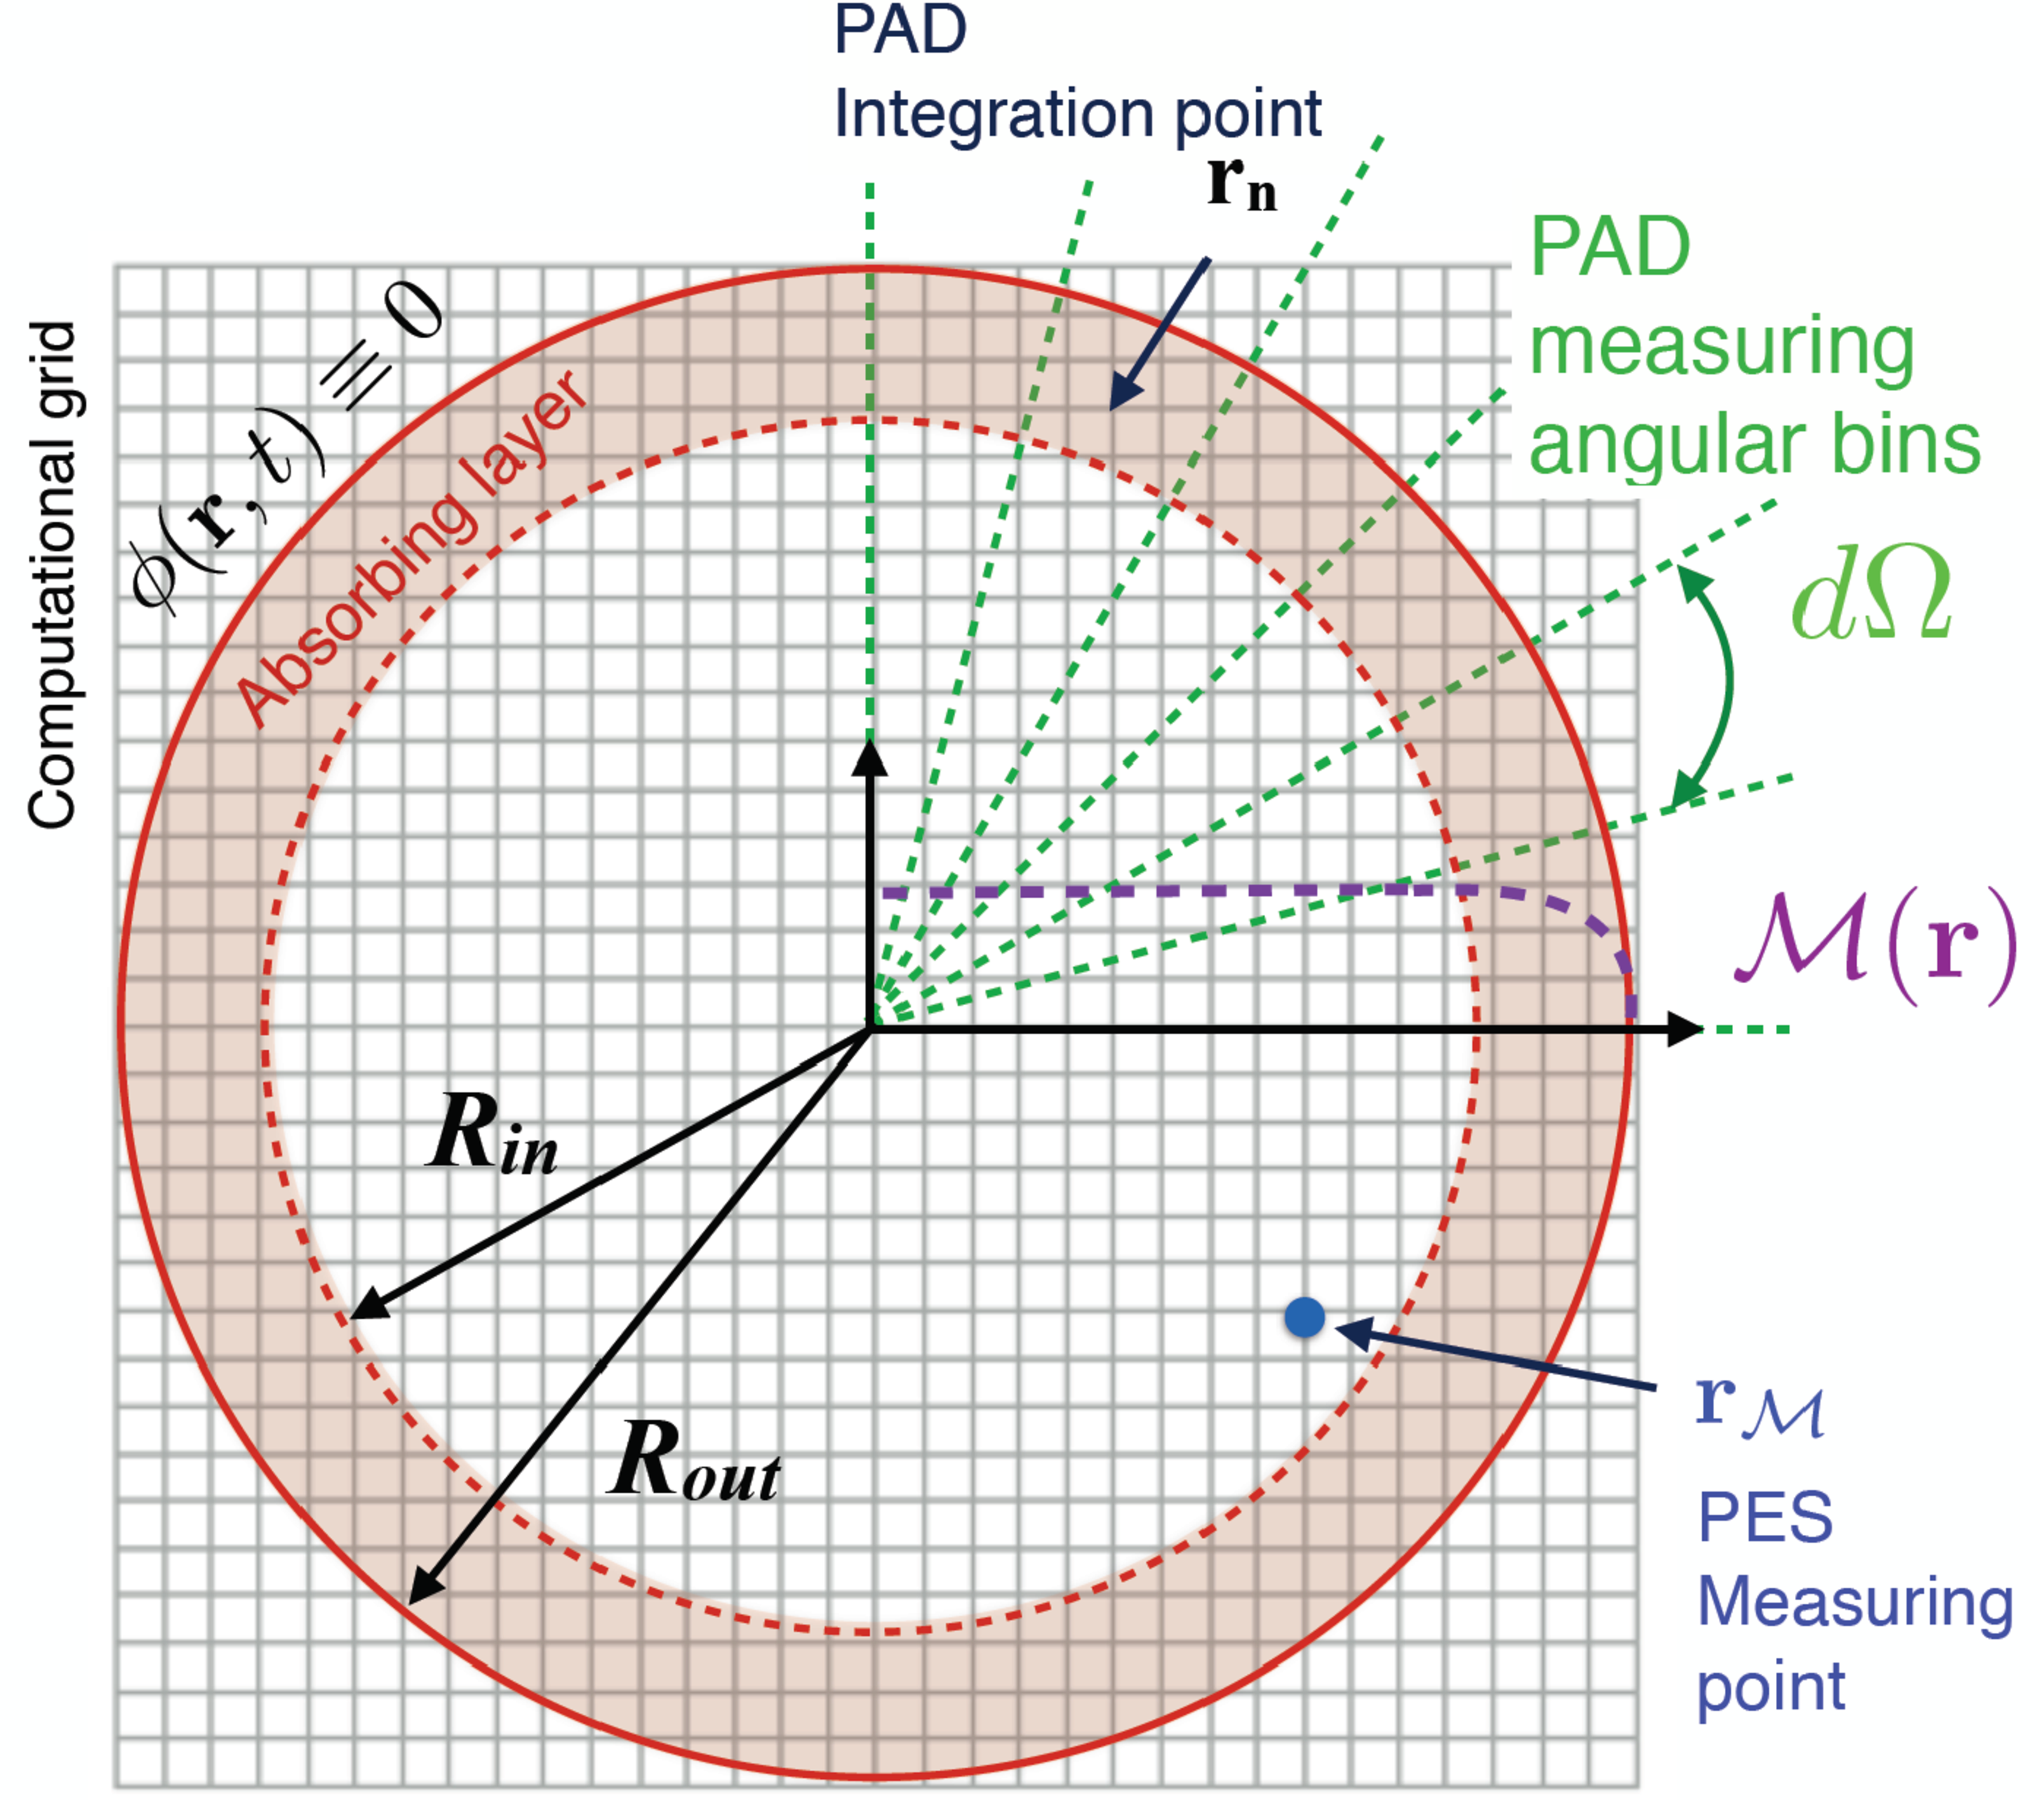
\includegraphics[width=0.7\linewidth]{schem_abso}}
%\centerline{\includegraphics[width=0.7\linewidth]{bounds}}
\caption{Schematic view of a coordinate-space grid with
absorbing bounds (ring zone), a sampling direction for accumulating PAD, and
measuring points $\mathbf{r}_\mathcal{M}$ for the PES.
 \label{fig:mask}}
\end{figure}
Proper handling of electron emission requires absorbing boundary
conditions. These are indicated by the ring area in the figure
covering here 3 grid points in each direction (actual calculations
typically use 6 and more points.) The absorption is performed in each time
step as~:
\begin{subequations}
\begin{eqnarray}
  \varphi(\mathbf{r},t)
  &\longrightarrow&
  \tilde\varphi(\mathbf{r},t\!+\!\delta t)
  =
  \hat{\mathcal{U}}_\mathrm{KS}(t\!+\!\delta t,t)\, \varphi(\mathbf{r},t)
  \quad,
\label{eq:KSpart}\\
  \varphi(\mathbf{r},t\!+\!\delta t)
  &=&
  \mathcal{M}(\mathbf{r})\, \tilde\varphi(\mathbf{r},t\!+\!\delta t)
  \quad,
\label{eq:maskact}
\\
  \mathcal{M}(\mathbf r)
  &=&
  \left\{\begin{array}{lll}
  1 & \mbox{for} &|\mathbf{r}|<R_\mathrm{in}
  \quad,
  \\
  \displaystyle
 \cos\left(
  \frac{|\mathbf{r}|-R_\mathrm{in}}{R_\mathrm{out}-R_\mathrm{in}}\frac{\pi}{2}
 \right)^{\gamma_\mathcal{M}}
  &\mbox{for}&
  R_\mathrm{in}<|\mathbf{r}|<R_\mathrm{out}
  \quad,
  \\
  0 
  &\mbox{for}&
  R_\mathrm{out}<|\mathbf{r}|
  \quad.
  \end{array}\right.
\label{eq:mask}
\end{eqnarray}
\end{subequations}
%
First comes one standard KS step \PGRfoot{Crossref to numerical
  section.} expressed here in terms of the TDLDA propagator
$\hat{\mathcal{V}}_\mathrm{KS}$, which yields the intermediate wave
function $\tilde\phi(\mathbf{r},t\!+\!\delta{t})$. This is followed by
the action (\ref{eq:maskact}) of the mask function $\mathcal{M}$
defined in Eq.(\ref{eq:mask}), which removes gradually any amplitude
towards the bounds. We use here a spherically symmetric mask. The
spherical profile is helpful to minimize griding artifacts when
computing angular distributions \cite{Poh04b} (simpler rectangular
masks may be used if PAD are not of interest). The absorbing bounds
steadily reduce the norm of the wave functions from the inner mask
radius $R_\mathrm{in}$ to the outer one $R_\mathrm{out}$.  This looks
simple and straightforward. However, the mask technique is not
perfect. One will always encounter a small amount of reflected flow,
particularly for electrons with low kinetic energy. One can minimize
the back-flow by proper choice of the exponent $\gamma_\mathcal{M}$
entering the mask profile, see Eq.~(\ref{eq:mask}). This depends,
however, on the actual numerics (number of absorbing points, size of
time step), for a detailed discussion see \cite{Rei06c}. Typical
values of $\gamma_\mathcal{M}$ are of order $1/8$ or lower.


\subsection{Observables}
\label{sec:observ}


\subsubsection{Energies}
\label{sec:energies}

The total binding energy $E(N_\mathrm{el},{\bf R}^{(N_\mathrm{ion})})$,
depending in ionic configuration and electron number, is a most
prominent observable and it is naturally result of any calculations
with energy-density functionals.  Comparison with measurements is
usually done in terms of differences of energies, e.g., the monomer
separation energy as the adiabatic energy difference
%
$E_\mathrm{mon}=E(N_\mathrm{el},{\bf R}^{(N_\mathrm{ion})})
            -E(N_\mathrm{el}-1,{\bf R}^{(N_\mathrm{ion}-1)})$
%
where the both energies are to be taken from fully relaxed ionic
configurations, or the vertical ionization potential
(IP)
%
$E_\mathrm{IP}=E(N_\mathrm{el},{\bf R}^{(N_\mathrm{ion})})
            -E(N_\mathrm{el}-1,{\bf R}^{(N_\mathrm{ion})})$
%
where the new electronic state in the $N_\mathrm{el}-1$ system has
relaxed but the ions are kept in their original configuration.


As a byproduct of mean field calculations, one obtains also the series
of s.p. energies $\varepsilon_\alpha$.  But it is known that
$\varepsilon_\alpha$ from (TD)LDA are spoiled by the self-interaction
error. This defect can be cured by a SIC, see section \ref{sec:SIC},
after which the set of $\varepsilon_\alpha$ provides a fair map of
electron separation energies, particularly of the IP
\cite{Leg02,Klu13}. Experimental data on s.p. energies are mainly the
IP and the sequence of peaks in PES from one-photon processes with
weak laser pulses.  Note that the latter can also be computed directly
from TDLDA and analysis of emitted electrons, see section
\ref{sec:PES}, which is anyway compulsory above the regime of weak
pulses. Besides comparison with data, the s.p. energies are very
instructive observables for theoretical interpretation as, e.g.,
analyzing electronic shell structure \cite{Hee93,Bra93}.

Other ``theoretical'' observables are the separate energy
contributions, particularly potential and kinetic energy.  The latter
can be used to define an ``intrinsic kinetic energy''
$E_\mathrm{kin,intr}$ which characterizes the amount of internal, so
to say thermal, kinetic excitation of the electron cloud. This is a
quantity which will play a key role in the model for dissipation
outlined in section \ref{sec:RTA}.


\subsubsection{Densities and shapes}
\label{sec:shapes}

Energy-density functional produce also the electronic local density
$\varrho(\mathbf{r})$ as natural outcome.  This together with the
ionic configuration $\{\mathbf{R}_I\}$ constitutes the shape of a
system and they do that in all detail which is in most cases
overwhelmingly much information. The gross structure of a shape is
well sorted in terms of its multipole moments. 
Leading quantity is the is the root-mean-square (r.m.s.) radius
which reads for the electrons
\begin{subequations}
\label{eq:moments}
\begin{equation}
  r_\mathrm{rms}
  =
  \sqrt{\frac{\int d^3r\,\varrho(\mathbf{r})\,r^2}{N}}
  \quad.
\end{equation}
The further multipoles
are best quantified in terms of dimensionless moments
\begin{equation}
  \alpha_{lm}
  =
  \frac{4\pi}{5}
  \frac{\int d^3r\,\varrho(\mathbf{r})\, r^lY_{lm}}
       {N_\mathrm{el}r_\mathrm{rms}^l}
  \quad.
\label{eq:def_dimless}
\end{equation}
\end{subequations}
Axially symmetric systems are distinguished by
$\alpha_{lm\!\neq\!0}=0$.  The appearance of $\alpha_{lm\!\neq\!0}\neq
0$ can have two causes: first, the system is not aligned along its
principal axes, and second, there is a true breaking of axial
symmetry. The first action is then to rotate the system such that the
$z$-axis is identical with one principal axis of the cluster. Axial
symmetry is truly broken if we then still find some
$\alpha_{lm\!\neq\!0}\neq 0$. As far as the quadrupole is concerned,
the only remaining case is $\alpha_{22}=\alpha_{2\!-\!2}\neq 0$
signaling triaxial shapes. One often regroups the quadrupole
deformation parameters into total deformation $\beta_2$ and
triaxiality $\gamma$ as
\begin{equation}
  \beta_2
  =
  \sqrt{\sum_m\alpha_{2m}^2}
  \quad,\quad
  \gamma
  =
  \mbox{atan}\left(\frac{\sqrt{2}\alpha_{22}}{\alpha_{20}}\right)
  \quad.
\label{eq:triax}
\end{equation}
This convention has been originally introduced to characterize shapes
of nuclei \cite{Hil53} and has been taken over for clusters at several
places, e.g. \cite{Lau91,Rei95b,Yan95}. It is to be noted that
$\gamma=0^o$ as well as $\gamma=60^o$ represent axially symmetric
shapes. The case $\gamma=0^o$ corresponds  to prolate shapes and
$\gamma=60^o$ to oblate ones.

The same definitions apply to ionic shapes if we replace $\int
d^3r\,\varrho(\mathbf{r})\,r^lY_{lm}(\Omega_r)
\longrightarrow\sum_IR_I^lY_{lm}(\Omega_R)$ in
Eqs. (\ref{eq:moments}).
In case of ions, 
the quadrupole shape is often alternatively characterized by the
moments of inertia
\begin{equation}
  I_{ii}=M\sum_I\left(R^2_{\mbox{}}-R_i^2\right)
  \quad\mbox{for}\quad
  i\in\{x,y,z\}
  \quad,
\end{equation}
to be evaluated in the frame of principal axes of the cluster ions.  The
mass $M$ is here the ion mass.
The relation between these moments of inertia and the 
above dimensionless quadrupole moments is
\begin{subequations}
\begin{eqnarray}
  r_\mathrm{rms}
  &=&
  \sqrt{\frac{I_{xx}+I_{yy}+I_{zz}}{2MN}}
  \quad,
\\
  \alpha_{20}
  &=&
  \frac{4\pi}{5}\sqrt{\frac{5}{16\pi}}
  \frac{\langle I_{xx}+I_{yy}-2I_{zz}\rangle}{NMr^2}
  \quad,
\\
  \alpha_{22}+\alpha_{2-2}
  &=&
  \frac{4\pi}{5}\sqrt{\frac{15}{8\pi}}
  \frac{\langle I_{yy}-I_{xx}\rangle}{NMr^2}
  \quad.
\end{eqnarray}
\end{subequations}

Radius and multipole moments are at first glance static observables
used to characterize cluster structure. But they are also important
ingredients to evaluate response properties as will become apparent in
the next two sections.


\subsubsection{Polarizability}
\label{sec:comppol}

The static polarizability is a key observable of atoms, molecules, and
clusters.  its computation is straightforward.  We discuss it here the
most important case of dipole polarizability $\alpha_D$.  One applies
a static external dipole field
$V_\mathrm{ext}(\mathbf{r})=e\mathbf{E}_0\!\cdot\!{\bf r}$ and
performs static calculations for a couple of $\mathbf{E}_0$.  This
delivers a dipole momentum $\bar{\bf D}=\langle e\mathbf{r}\rangle$ as
a function of $\mathbf{E}_0$. The tensor of static dipole
polarizability is then
\begin{equation}
  (\alpha_D)_{ij}
  =
  \frac{\partial\bar{D}_i}{\partial{E}_{0,j}}\Big|_{\mathbf{E}_0=0}
  \quad.
\label{eq:comppolar}
\end{equation}
The polarizability matrix simplifies if the system has spatial
symmetries. For example, an axially symmetric system aligned with the $z$-axis
has $(\alpha_D)_{xz}=(\alpha_D)_{yz}=(\alpha_D)_{xy}=0$ and
$(\alpha_D)_{xx}=(\alpha_D)_{yy}$ and a spherically symmetric system
has additionally $(\alpha_D)_{xx}=(\alpha_D)_{zz}$.

\subsubsection{Optical response}
\label{sec:specan}

Optical response is a key observable in cluster physics.  In the limit
of long wavelengths, the photon field at the system site is related
the dipole momentum $\mathbf{D}=\mathbf{r}$ where $\mathbf{r}$ is
taken with respect to the center-of-mass of the electron cloud.  With
the given code, the dipole excitation strength can be computed by
spectral analysis of the dipole response to an instantaneous dipole
excitation of the system.  To that end, one starts from a well relaxed
ground state and applies the instantaneous initial excitation by a
small dipole boost
\begin{subequations}
\begin{equation}
  \varphi_\alpha(\mathbf{r},t\!=\!0)
  =
  e^{\mathrm{i}\mathbf{p}_0\cdot\mathbf{r}}
  \varphi_{\alpha,\mathrm{g.s.}}(\mathbf{r})
\end{equation}
where $\mathbf{p}_0$ is a (small) boost momentum.  One then propagates
electrons with TDLDA and samples a protocol of the dipole momentum
\begin{equation}
  {\bf D}(t)
  =
  \int d{\bf r}\,{\bf r}\rho({\bf r},t)
  \quad.
\end{equation}
After a sufficient time ($T_\mathrm{max}$), one Fourier transforms the
dipole signal with an appropriate window function $\mathcal{W}(t)$ and
finally obtains the spectral strength $S_{D_i}(\omega)$ in $x$, $y$,
or $z$ directions and corresponding spectral power $\mathcal{P}_{D_i}$
as\PGRfoot{The dipole strength function, also known as dynamic
  polarizability, is in principle a tensor as $\alpha_D$ is. Should we
address that or better restrict discussion to one coordinate only?}
\begin{eqnarray}
  S_{D_i}(\omega)
  &=&
  \Im\{\tilde{D}_i(\omega)\}
  \quad,\quad
  \tilde{D}_i(\omega)
  =
  \int dt\,\mathcal{W}(t)\,e^{\imath\omega t}D_i(t)
  \quad,
\\
  \mathcal{P}_{D_i}(\omega)
  &=&
  |\tilde{D}_i(\omega)|^2
  \quad.
\end{eqnarray}
\end{subequations}
The maximum possible {spectral resolution} is given by
$\delta\omega=2\pi/T_\mathrm{max}$.
%
The window function $\mathcal{W}(t)$ serves to attenuate the dipole
signal toward the end point $T_\mathrm{max}$ in order to avoid
artifacts from non-zero $\mathbf{D}(T_\mathrm{max})$
\cite{Pre92}. Useful windows are
$\mathcal{W}(t)=\cos^{2n}(t\pi/(2T_\mathrm{max})$ where $n$ is an
integer number. The choice $n=1$ produces often still a bit rough
$\Im\{\tilde{D}_i(\omega)\}$ while $n=2$ performs usually satisfyingly
well.  It is interesting to note that this treatment in connection
with absorbing boundary conditions (see section \ref{sec:abso}) allows
to compute correctly the escape width of spectral states lying in
the electron continuum. For details of spectral analysis and variants
thereof see \cite{Cal97b}.

Spectral analysis can equally well be performed with other
observables, as e.g. higher multipoles, spin modes etc. The full
TDLDA furthermore allows one to go beyond the linear regime. The more
appropriate observable is then the power spectrum.


The same principles of spectral analysis apply, of course, also for
computing the vibrational spectra of clusters. Here we concentrate on
the MD part of TDLDA-MD.  The analyzing times are, of course, to be
taken much longer to supply sufficient spectral resolution for the
excitations in the meV range, characteristic of ionic vibrational
states, and the ionic multipole momenta ought to be used for the
spectral analysis of ionic motion \cite{Rei02d}.



\subsubsection{Ionization}
\label{sec:ionization}

Absorbing boundary conditions as explained in section \ref{sec:abso}
provide a pertinent picture of electron emission.  There are several
observables associated with emission from (photo-)excited systems: net
ionization, photo-electron angular distribution (PAD), and
photo-electron spectra (PES). We discuss them in the next three
sections.

The first observable is the total ionization, i.e. the number of
escaped electrons $N_\mathrm{esc}$. This can be computed simply from
the, now decreasing, single-particle norms as~:
\begin{equation}
  N_\mathrm{esc}(t)
  =
  \sum_{i=1}^N N_{\mathrm{esc},i}(t)
  \quad,\quad
  N_{\mathrm{esc},i}(t)
  =
  1-\sum_i \langle \varphi_i(t)|\varphi_i(t)\rangle
  \quad.
\label{eq:nesc}
\end{equation}
This shows that we have access to even more than the mere net
ionization. Indeed each $1-N_{\mathrm{esc},i}$ yields the depletion of
s.p. state $i$ separately. Both, total ionization and detailed level
depletion are very instructive observables \cite{Din12c}.


\subsubsection{Photo-electron angular distribution (PAD)}
\label{sec:pad}


The angular distributions
$\mathrm{d}\sigma/\mathrm{d}\Omega(\vartheta,\phi)$ are evaluated in
angular segments labeled by the azimuthal angle $\vartheta $ and the
polar angle $\phi$, see Fig.~\ref{fig:mask}. The reference frame for
these two angles is usually the $z$ axis identical with the laser
polarization axis.  We
collect all probability which was removed by the absorption step
(\ref{eq:maskact}) and accumulate it.  A straightforward collection of
grid points in a segment tends to produce noisy results because the
number of grid points per segment fluctuates. We therefore associate
with each grid point a smoothing function $\mathcal{S}(\mathbf{r})$
which distributes the strength over a vicinity of order of grid
spacing.  This suffices to produce acceptable smooth distributions.
The PAD is thus computed as~:
\begin{subequations}
\label{eq:PADfixed}
\begin{eqnarray}
%  \frac{d\sigma}{d\Omega}(\vartheta,\varphi)
  \mathcal{A}(\vartheta,\phi)
  &=&
  \sum_{i=1}^N\mathcal{A}^{(i)}(\vartheta,\phi)
  \quad,
\\
  \mathcal{A}^{(i)}(\vartheta,\phi)
  &=&
  \sum_{\mathbf{n}\in\mbox{abs.b.c.}}
  \int \textrm dr\,r^2\,\mathcal{S}(r\mathbf{e}_r-\mathbf{r}_\mathbf{n})
   \, n_{\mathrm{esc},i}(\mathbf{r}_\mathbf{n})
  \quad,
\\
  \mathcal{W}(\mathbf{r})
  &=&
  \frac{\mbox{max}(\Delta x-|x|,0)}{\Delta x} \, 
  \frac{\mbox{max}(\Delta y-|y|,0)}{\Delta y} \,
  \frac{\mbox{max}(\Delta z-|z|,0)}{\Delta z}
  \quad,
\\
  n_{\mathrm{esc},i}(\mathbf{r}_\mathbf{n})
  &=&
  \int \textrm dt\,\left|\varphi_i(\mathbf{r}_\mathbf{n},t)\right|^2
  \left[1-\mathcal{M}(\mathbf{r}_\mathbf{n},t)\right]
  \quad,
\end{eqnarray}
\end{subequations}
where $\mathbf{e}_r=\left(\sin\vartheta\cos\phi,
\sin\vartheta\sin\phi,\cos\vartheta\right)$ is the unit vector in the
direction of the wanted angles. The smoothing is done by simple tent
functions which comply with the integration rule used in the
normalization.  The angular segments in Fig.~\ref{fig:mask} try to
symbolize this smoothing which collects (weighted) information in the
vicinity of a ray. The above recipe applies to state specific PAD
$\mathcal{A}_i$ as well as the total PAD
$\mathcal{A}\equiv\mathrm{d}\sigma/\mathrm{d}\Omega(\vartheta,\phi)$.


\subsubsection{Photo-emission spectra (PES)}
\label{sec:pes}


The PES can be deduced from the temporal phase oscillations of the
wave functions $\varphi(\mathbf{r}^{(v)}_\mathcal{M},t)$ at measuring
points $\mathbf{r}_\mathcal{M}$ close to the absorbing bounds
\cite{Poh00}.  The result for the PES sampled at
$\mathbf{r}_\mathcal{M}$ is
\begin{subequations}
\label{eq:PESformula}
\begin{eqnarray}
  \mathcal{Y}(E_\mathrm{kin},\Omega_\mathcal{M})
  &=&
  \sum_\alpha w_\alpha
  \mathcal{Y}_\alpha(E_\mathrm{kin},\Omega_\mathcal{M})
  \quad,
\\
  \mathcal{Y}_\alpha(E_\mathrm{kin},\Omega_\mathcal{M})
%  \propto
%  \left|\widetilde{\varphi}^{(v)}_0(\sqrt{2\omega})\right|^2
  &=&
  \left|
  \!\int\!\frac{dt}{\sqrt{2\pi}}\,e^{\mathrm{i}E_\mathrm{kin}t
              -\mathrm{i}\delta q\sqrt{2E_\mathrm{kin}}
              +\mathrm{i}\delta\Omega
              +\mathrm{i}E_0F(t)\mathbf{e}_E\cdot\mathbf{r}_\mathcal{M}}
               \varphi(\mathbf{r}_\mathcal{M},t)
  \right|^2
  \;,
\label{eq:solve-wf}
\\
  \delta q(t)
  &=&
  E_0 \int_{0}^t\mathrm dt'\,F(t')
  \quad,
\label{eq:delq}\\
  \delta\Omega(t)
  &=&
  \frac{E_0^2}{2}\int_{0}^t\mathrm dt'\,F(t')^2
  \quad,
\label{eq:delOmega}
\end{eqnarray}
\end{subequations}
where $\mathbf{e}_E$ is the direction of (linear) polarization of the
electrical field, $\Omega_\mathcal{M}$ the space angle associated with
$\mathbf{r}_\mathcal{M}$, and
$F(t)=\int{d}t'\,f(t')\exp{(-\mathrm{i}\omega_\mathrm{las}t')}$ the
time integrated laser pulse envelope introduced in
Eq.~(\ref{eq:laserp}).  This form applies for the wavefunction
$\varphi(\mathbf{r}_\mathcal{M},t)$ in space gauge as computed in the
code. Note that the formula does not only give the total PES, but also
the PES $\mathcal{Y}_\alpha$ for emission specifically from state
$\alpha$.

A detailed derivation of Eqs. (\ref{eq:PESformula}) is found in
\cite{Din13a}.  We summarize here the ideas behind that compact
formula.  It is deduced under the assumption that the measuring point
$\mathbf{r}_\mathcal{M}$ is sufficiently far away from the system
(placed around $\mathbf{r}=0$) such that that outgoing electron wave
has direction
$\mathbf{e}_{\mathbf{k}}=\mathbf{e}_\mathcal{M}=\mathbf{r}_\mathcal{M}/r_\mathcal{M}$.
We expand the wavefunction at $\mathbf{r}_\mathcal{M}$ into outgoing
waves with direction $\mathbf{e}_{\mathbf{k}}$ and momenta
$k>0$. These are plane waves
$e^{\mathrm{i}k\mathbf{e}_{\mathbf{k}}\cdot\mathbf{r}_\mathcal{M}}$
for weak fields and for stronger fields the corresponding electron
waves in the time-dependent photon field (Volkov states).  The fact
that we have only outgoing waves in one direction allows to identify
uniquely energy and momentum as
$\mathbf{k}=\mathbf{e}_{\mathbf{k}}\sqrt{2E_\mathrm{kin}}$.  The
energy is read off from the phase oscillations of
$\varphi(\mathbf{r}^{(v)}_\mathcal{M},t)$ and the direction
$\mathbf{e}_{\mathbf{k}}\Rightarrow\Omega_\mathrm{M}$ from the
position of the measuring point.

The formula (\ref{eq:PESformula}) applies for weak and for strong
field, but still fails for extremely strong fields. The limits of
validity depend on system and time structure of the pulse.  To give an
order of magnitude, a intensity for long photon pulses impinging on Na
clusters is $I\approx\times{10}^{15}$W/cm$^2$. For details see
\cite{Din13a}.


\section{The structure of the TDLDA package}
\label{sec:TDLDAnum}


\subsection{The TDLDA calling tree}
\label{sec:TDLDAtree}

The TDLDA packages is a rather complex collection of routines.  Thus
the tree structure of the code is sketched only at the major level of
callings and is presented in three separate diagrams: the main routine
with all initializations and two calls to the major drivers for static
and dynamic calculations in diagram \ref{fig:tree_main}, the static
driver in diagram \ref{fig:tree_static}, and the dynamic driver in
\ref{fig:tree_dyn}.
\begin{figure}
\centerline{\fbox{
\begin{picture}(122,158)(5,-146)
\put(10,8){\mbox{\tt main}}
\put(11,7){\line(0,-1){147}}
 \put(50,1){\mbox{\large general initializations}}
   \put(20,-4){\mbox{\tt cpu\_time,  init\_parallele, init\_simann}}
   \put(11,-3){\line(1,0){8}}
   \put(20,-8){\mbox{\tt  initnamelists, checkoptions}}
   \put(11,-7){\line(1,0){8}}
   \put(20,-12){\mbox{\tt init\_baseparams, iparams}}
   \put(11,-11){\line(1,0){8}}
   \put(20,-16){\mbox{\tt iperio, changeperio}}
        \put(90,-16){\mbox{$\leftrightarrow$ PsP tables}}
   \put(11,-15){\line(1,0){8}}
   \put(20,-20){\mbox{\tt init\_grid, init\_fields}}
   \put(11,-19){\line(1,0){8}}
   \put(20,-24){\mbox{\tt init\_radmatrix}}
        \put(90,-24){\mbox{$\leftrightarrow$ tables for SIC}}
   \put(11,-23){\line(1,0){8}}
   \put(20,-28){\mbox{\tt ocoption, init\_output}}
   \put(11,-27){\line(1,0){8}}
   \put(20,-32){\mbox{\tt init\_jellium, initions}}
   \put(11,-31){\line(1,0){8}}
   \put(20,-36){\mbox{\tt pseudo\_external}}
        \put(90,-36){\mbox{$\leftrightarrow$ read explicit PsP}}
   \put(11,-35){\line(1,0){8}}
   \put(20,-40){\mbox{\tt initwf}}
   \put(11,-39){\line(1,0){8}}
   \put(20,-44){\mbox{\tt init\_homfield}}
   \put(11,-43){\line(1,0){8}}
   \put(20,-48){\mbox{\tt timer, init\_boxpara}}
   \put(11,-47){\line(1,0){8}}
 \put(50,-55){\mbox{\large static part}}
   \put(20,-60){\mbox{\tt init\_fsicr}}
   \put(11,-59){\line(1,0){8}}
   \put(20,-64){\fbox{\tt statit}}
   \put(11,-63){\line(1,0){8}}
   \put(20,-68){\mbox{\tt simann}}
   \put(11,-67){\line(1,0){8}}
   \put(20,-72){\mbox{\tt afterburn}}
   \put(11,-72){\line(1,0){8}}
 \put(50,-79){\mbox{\large dynamic part}}
   \put(20,-84){\mbox{\tt init\_absbc, init\_abs\_accum, initmeasurepoints}}
   \put(11,-83){\line(1,0){8}}
   \put(20,-88){\mbox{\tt init\_dynprotocol, evaluate}}
   \put(11,-87){\line(1,0){8}}
   \put(20,-92){\mbox{\tt init\_fsic, init\_scattel{\rm(??)}}}
   \put(11,-91){\line(1,0){8}}
   \put(20,-96){\mbox{\tt init\_dynwf}}
   \put(11,-95){\line(1,0){8}}
   \put(20,-100){\mbox{\tt restart2, addcluster}}
   \put(11,-99){\line(1,0){8}}
   \put(20,-104){\mbox{\tt calclocal, calc\_sic, calcpseudo}}
   \put(11,-103){\line(1,0){8}}
   \put(20,-108){\mbox{\tt dyn\_mfield, fermi\_init, info}}
   \put(11,-107){\line(1,0){8}}
   \put(20,-112){\mbox{\tt mergetabs, ordo\_per\_spin}}
   \put(11,-111){\line(1,0){8}}
   \put(20,-116){\mbox{\tt calc\_proj, calc\_projFine}}
   \put(11,-115){\line(1,0){8}}
   \put(20,-120){\mbox{\tt mpi\_barrier}}
   \put(11,-119){\line(1,0){8}}
   \put(20,-124){\mbox{\tt rhointxy, rhointxz, rhointyz}}
   \put(11,-123){\line(1,0){8}}
   \put(20,-128){\mbox{\tt lffirststep}}
   \put(11,-127){\line(1,0){8}}
   \put(20,-132){\mbox{\tt open\_protok\_el, analyze\_elect}}
   \put(11,-131){\line(1,0){8}}
   \put(20,-136){\fbox{\tt dyn\_propag}}
   \put(11,-135){\line(1,0){8}}
   \put(20,-141){\mbox{\tt mpi\_finalize}}
   \put(11,-140){\line(1,0){8}}
\end{picture}
}}
\caption{\label{fig:tree_main}
Schematic calling tree for the main routine in {\tt main.F90}.
The calling trees for the two major 
subroutines in framed boxes are explained in
subsequent figures \ref{fig:tree_static} and  \ref{fig:tree_dyn}.
}
\end{figure}


\begin{figure}
\centerline{\fbox{
\begin{picture}(122,66)(5,-62)
\put(10,0){\mbox{\tt static}}
\put(11,-1){\line(0,-1){58}}
   \put(20,-4){\mbox{\tt calcrhor}}
   \put(11,-3){\line(1,0){8}}
   \put(20,-8){\mbox{\tt falr, solv\_possion}}
   \put(11,-7){\line(1,0){8}}
   \put(20,-12){\mbox{\tt calcpseudo, static\_mfield}}
   \put(11,-11){\line(1,0){8}}
   \put(20,-16){\mbox{\tt pricm, infor, prifld}}
   \put(11,-15){\line(1,0){8}}
   \put(20,-20){\mbox{\tt sstep}}
   \put(11,-19){\line(1,0){8}}
   \put(21,-21){\line(0,-1){22}}
      \put(30,-24){\mbox{\tt cpu\_time, system\_clock}}
      \put(21,-23){\line(1,0){8}}
      \put(30,-28){\mbox{\tt exchgr, subtr\_sicpot}}
      \put(21,-27){\line(1,0){8}}
      \put(30,-32){\mbox{\tt nonlocalr}}
      \put(21,-31){\line(1,0){8}}
      \put(30,-36){\mbox{\tt rftf, rfftback, rkin3D}}
      \put(21,-35){\line(1,0){8}}
      \put(30,-40){\mbox{\tt project, givens}}
      \put(21,-39){\line(1,0){8}}
      \put(30,-44){\mbox{\tt schmidt, reocc}}
      \put(21,-43){\line(1,0){8}}
   \put(20,-48){\mbox{\tt prifldz, pri\_pstat, printfield}}
   \put(11,-47){\line(1,0){8}}
   \put(20,-52){\mbox{\tt localizer, mtv\_field}}
   \put(11,-51){\line(1,0){8}}
   \put(20,-56){\mbox{\tt resume, rsave}}
   \put(11,-55){\line(1,0){8}}
   \put(20,-60){\mbox{\tt infor\_sic, diag\_lagr}}
   \put(11,-59){\line(1,0){8}}
\end{picture}
}}
\caption{\label{fig:tree_static}
Schematic calling tree for the static driver routine in {\tt static.F90}.
}
\end{figure}


\begin{figure}
\centerline{\fbox{
\begin{picture}(122,70)(5,-66)
\put(10,0){\mbox{\tt dyn\_propag}}
\put(11,-1){\line(0,-1){62}}
   \put(20,-4){\mbox{\tt stimer, print\_densdiff, savings}}
   \put(11,-3){\line(1,0){8}}
   \put(20,-8){\fbox{\tt rta}}
   \put(11,-7){\line(1,0){8}}
        \put(90,-8){\mbox{$\leftrightarrow$ see section \ref{sec:RTA}}}
   \put(20,-12){\mbox{\tt init\_occ\_target, init\_psitarget}}
   \put(11,-11){\line(1,0){8}}
   \put(20,-16){\mbox{\tt tstep\_exp, CrankNicholson\_exp}}
   \put(11,-15){\line(1,0){8}}
   \put(20,-20){\mbox{\tt tstep}}
   \put(11,-19){\line(1,0){8}}
   \put(21,-21){\line(0,-1){18}}
      \put(30,-24){\mbox{\tt cpu\_time, system\_clock}}
      \put(21,-23){\line(1,0){8}}
      \put(30,-28){\mbox{\tt nonlocstep}}
      \put(21,-27){\line(1,0){8}}
      \put(30,-32){\mbox{\tt kinprop, fftf, fftback}}
      \put(21,-31){\line(1,0){8}}
      \put(30,-36){\mbox{\tt eval\_unitrot}}
      \put(21,-35){\line(1,0){8}}
      \put(30,-40){\mbox{\tt dyn\_meanfield, escmask, checkzeroforce}}
      \put(21,-39){\line(1,0){8}}
   \put(20,-44){\mbox{\tt rhointxy, rhointxz, rhointyz, testcurrent}}
   \put(11,-43){\line(1,0){8}}
   \put(20,-48){\mbox{\tt itstep, itstepv, enerkin\_ions, reset\_ions}}
   \put(11,-47){\line(1,0){8}}
   \put(20,-52){\mbox{\tt calc\_pseudo, calclocal, calc\_sic}}
   \put(11,-51){\line(1,0){8}}
   \put(20,-56){\mbox{\tt calc\_proj, calc\_projFine}}
   \put(11,-55){\line(1,0){8}}
   \put(20,-60){\mbox{\tt analyze\_elect, analyze\_ions, energ\_ions}}
   \put(11,-59){\line(1,0){8}}
   \put(20,-64){\mbox{\tt mpi\_barrier}}
   \put(11,-63){\line(1,0){8}}
\end{picture}
}}
\caption{\label{fig:tree_dyn}
Schematic calling tree for the static driver routine in {\tt dynamic.F90}.
The routine in the framed box is explained in great detail in section
\ref{sec:RTA}. 
}
\end{figure}

\subsection{The TDLDA subroutines in detail}
\label{eq:detailsTDLDA}


\PGRcomm{Here is to come a detailed description of the subroutines
  similar as for RTA in \ref{eq:details}, but here for the LDA part.
Only one example is given as appetizer. The problem is that it cost
enormous amounts of space to present all routines and functions at that
level of detail. We should shift that to the
supplementary material. It will comes there anyway if we decide to
transfer all these details to {\tt doxygen}.
}

\subsubsection*{\tt SUBROUTINE coul\_mfield(rho)}
\begin{tabular}{lcl}
 {\tt rho(1:2*kdfull2)} & in/out & \\ density for which Coulomb field
 is computed
\end{tabular}
\\[4pt]
Computes Coulomb potential for given density by invoking
Poisson solver.
Th emerging coulomb potential is communicated as {\tt chpcoul}
via module {\tt params}.
In case of dielectric external media, adds pseudo-density for image
charge.
\\
\PGRcomm{Why is {\tt rho} also {\tt INTENT OUT}? Is all {\tt
    1:2*kdfull2} used or only the first block {\tt 1:kdfull2}?}



%\subsubsection*{\tt }
%\begin{tabular}{lcl}
% {\tt } & &\\
%\end{tabular}
%\\[4pt]




\section{Relaxation-time approximation (RTA)}
\label{sec:RTA}

\subsection{The formal background of RTA}

The quantum Boltzmann equation is the quantum mechanical
counterpart of the
semiclassical Vlasov-Uehling-Uhlenbeck equation \cite{Ber88,Abe96}.
It complements the self-consistent TDLDA propagation 
of the one-body density matrix $\hat{\rho}$ by
dynamical correlations through a collision term. It reads in
general \cite{Rei85f,Goe86a}
%\begin{eqnarray}
$\mathrm{i}\partial_t\hat{\rho}
  -
  \big[\hat{h},\hat{\rho}\big]
  =
  \hat{I}[\hat{\rho}]
%  \quad.
$
%\label{eq:EoMfull}
%\end{eqnarray}
where the left hand side contains the mean-field propagation. the
$\hat{I}$ at the right-hand side consists stands for the
quantum-mechanical collision term which, however, is extremely hard to
handle for finite Fermion systems. A great simplification can be
achieved by the relaxation-time approximation (RTA) which was used
successfully in a wide variety of homogeneous systems
\cite{Pin66,Ash76}. The RTA equations for the present case of finite
Fermion systems read \cite{Rei15a}
\begin{subequations}
\label{eq:EoMbasic}
\begin{eqnarray}
  \partial_t\hat{\rho}
  &=&
  -\mathrm{i}\big[\hat{h},\hat{\rho}\big]
  -
  \frac{1}{\tau_\mathrm{relax}}
  \left(\hat{\rho}-\hat{\rho}_\mathrm{eq}[\varrho,\mathbf{j},E_\mathrm{sp}]\right)
  \;,
\label{eq:EoMbasicrho}
\\
  \varrho(\mathbf{r},t)
  &=&
  \sum_\alpha \left|\phi_\alpha(\mathbf{r},t)\right|^2 W_\alpha
  \;,
\label{eq:locdens}\\
  \mathbf{j}(\mathbf{r},t)
  &=&
  \sum_\alpha W_\alpha\phi_\alpha^*(\mathbf{r},t)
     \frac{\stackrel{\rightarrow}{\nabla}-\stackrel{\leftarrow}{\nabla}}
          {2\mathrm{i}}
     \phi_\alpha(\mathbf{r})
  \;,
\label{eq:current}\\
  E_\mathrm{sp}
  &=&
  \sum_\alpha W_\alpha\varepsilon_\alpha
  \;,
\\  
  \frac{\hbar}{\tau_\mathrm{relax}}
  &=&
  {0.40}\frac{\sigma_{ee}}{r_s^2}\frac{{E}^*_\mathrm{intr}}{N}
  \;,\;
  r_s=\left(\frac{3\bar{\varrho}}{4\pi}\right)^{-1/3}
  \;,\;
  \sigma_{ee}=\sigma_{ee}(\bar{\varrho})
  \;,
\label{eq:relaxtime}
\end{eqnarray}
\end{subequations}
where $\hat{\rho}_\mathrm{eq}$ is the density operator of the thermal
equilibrium for local density $\varrho(\mathbf{r},t)$, current
distribution $\mathbf{j}(\mathbf{r},t)$. The reference energy should
be, in fact, the total energy $E(t)$ and computed from the actual
state $\hat{\rho}(t)$. We replace that by the simpler total s.p.
energy $E_\mathrm{sp}(t)$ which is legitimate because the difference
to $E$ is a functional of $\varrho(\mathbf{r})$ only, a quantity which
is kept frozen by construction.  The forms
(\ref{eq:locdens},\ref{eq:current}) hold for the diagonal
representation.  A crucial parameter is the relaxation time
$\tau_\mathrm{relax}$ which is taken over from semi-classical Fermi
liquid theory, for details see \cite{Rei15a}.  Key entries are: the
intrinsic (thermal) energy of the system $E^*_\mathrm{intr}$ (see
appendix \ref{app:eintr}), the actual number of particles $N$, the
in-medium electron-electron cross section $\sigma_{ee}$, the effective
Wigner-Seitz radius $r_s$ of the electron cloud, and the average
electron density $\bar{\varrho}$.  Note that $r_s$ and $\sigma_{ee}$
depend on an average density $\bar{\varrho}$ because a spatially
varying $\tau_\mathrm{relax}$ would be very cumbersome to implement in
a quantum mechanical expression.  The average density is deduced from
the r.m.s. radius $r$ of the actual electron cloud as
$\bar{\varrho}=(3N/(4\pi r^3))$\PGRfoot{Should we add that as
  displayed equation?}.

This RTA equation (\ref{eq:EoMbasic}) is rather involved because its
entries depend in various ways on the actual state $\hat{\rho}(t)$.
The most expensive piece is the instantaneous equilibrium density
operator
\begin{subequations}
\label{eq:DCMF}
\begin{equation}
  \hat{\rho}_\mathrm{eq}[\varrho,\mathbf{j},E]
  =
  |\phi_\alpha^\mathrm{(eq)}\rangle
  W_\alpha^\mathrm{(eq)}\langle\phi_\alpha^\mathrm{(eq)}|
\end{equation}
which minimizes LDA energy with constraint on the actual
$\varrho(\mathbf{r})$, $\mathbf{j}(\mathbf{r})$ and energy
$E_\mathrm{sp}$.  It is determined by the density-constrained
mean-field (DCMF) equation
\begin{eqnarray}
  \hat{h}_\mathrm{DCMF}[\varrho,\mathbf{j},E]\phi_\alpha^\mathrm{(eq)}
  &=&
  \varepsilon_\alpha^\mathrm{(eq)}\phi_\alpha^\mathrm{(eq)}
\\
  \hat{h}_\mathrm{DCMF}[\varrho,\mathbf{j}]
  &=&
  \hat{h}
  -
  \int d^3r\lambda(\mathbf{r})\hat{\varrho}(\mathbf{r})
  -
  \int d^3r\,\mbox{\boldmath$\lambda_j$}(\mathbf{r})\hat{\mathbf{j}}(\mathbf{r})
\nonumber\\
  &&\quad
  -
  \mu\int d^3r(\hat{\varrho}(\mathbf{r})-{\varrho}(\mathbf{r},t))^2
  -
  \mu_j\int
  d^3r\,(\hat{\mathbf{j}}(\mathbf{r})-{\mathbf{j}}(\mathbf{r},t))^2
\label{eq:hDCMF}
\end{eqnarray}
in combination with adjustment of particle number $N$ and s.p. energy
$E_\mathrm{sp}(t)$ through a Fermi distribution
\begin{eqnarray}
  W_\alpha^\mathrm{(eq)}
  &=&
  \frac{1}{1+
  \exp((\langle\phi_\alpha^\mathrm{(eq)}|\hat{h}|\phi_\alpha^\mathrm{(eq)}\rangle-\mu^\mathrm{(eq)})/T^\mathrm{(eq)})}
\label{eq:Fermi}\\
  &&\hspace*{-4em}
  \mu^\mathrm{(eq)}\leftrightarrow
  \sum_\alpha W_\alpha^\mathrm{(eq)}=N(t)
  \;,\;
  T^\mathrm{(eq)}\leftrightarrow
  \sum_\alpha W_\alpha^\mathrm{(eq)}
  \langle\phi_\alpha^\mathrm{(eq)}|\hat{h}|\phi_\alpha^\mathrm{(eq)}\rangle
  =
  E_\mathrm{sp}(t)
  \;.
\end{eqnarray}
\end{subequations}
%
Although cumbersome to evaluate, it is important to use exactly this
local, instantaneous equilibrium in the relaxation term. This
guarantees that the dissipative step conserves local density, 
current, and energy as it is mandatory for a good collision term
\cite{Gue88a}.


\subsection{Observables specific to relaxation}

Most of the observables computed with RTA are exactly the same as for
TDLDA, e.g., energy, density, excitation spectra, ionization, PES, or PAD.
New are observables related to the mixed character of the
one-body operator which is characterized by the occupation
numbers $W_\alpha$. 
A specific quantity in that respect is the 
entropy which is computed in diagonal representation
(\ref{eq:rhodiag}) by the standard expression \cite{Rei98aB}
\begin{equation}
  S
  =
  - \sum_\alpha\left[
    W_\alpha\log W_\alpha
    +
    (1\!-\!W_\alpha)\log (1\!-\!W_\alpha)
  \right]
\label{eq:entropy}
\end{equation}
in units of Boltzmann constant. 
It serves as a direct indicator of thermalization and allows to 
read off the typical time scale of relaxation processes. 



\subsection{Summary of the RTA procedure}
\label{sec:summaryRTA}




\begin{figure}
%\setlength\unitlength{0.91mm}
\thicklines
\begin{center}
%\begin{sideways}
\fbox{\small%\footnotesize
%\begin{picture}(130,92)(0,108)
\begin{picture}(132,175)(-5,-175)
\put(0,-5){\mbox{
\begin{minipage}[t]{8cm}
\begin{flushleft}
$\;$starting point: 
\\[4pt]
  $\hat{\rho}(t_0)
  =
  \sum_\alpha|\phi_\alpha(t_0)\rangle W_\alpha(t_0)\langle\phi_\alpha(t_0)|$
\end{flushleft}
\end{minipage}
}}
\put(5,-19){\encircle{1}}
\put(3,-11.5){\vector(0,-1){25}}
\put(6,-30){\fbox{\tt tstep}}
\put(7,-25){\mbox{mean-field propagation: 
$%\begin{array}{l}
 |\phi_\alpha^\mathrm{(mf)}\rangle=\hat{U}(t_1,t_0)|\phi_\alpha(t)\rangle
\;,\;
%\\
 W_\alpha^\mathrm{(mf)}=W_\alpha(t)=\mbox{const.}
%\end{array}
$
}}
\put(0,-40){\mbox{
  $ \hat{\rho}_\mathrm{mf} =\hat{\rho}_\mathrm{mf}(t_1) 
  =
  \sum_\alpha|\phi_\alpha^\mathrm{(mf)}\rangle 
  W_\alpha^\mathrm{(mf)}\langle\phi_\alpha^\mathrm{(mf)}|$
}}
\put(5,-46){\encircle{2}}
\put(6,-54.5){\fbox{\tt srhomat}}
\put(3,-41.5){\vector(0,-1){15}}
\put(0,-50){\mbox{
\begin{minipage}[t]{8cm}
\begin{flushleft}
\hspace*{1.8em}express $\phi$ and $W$ through natural orbitals
\\[20pt]
  $\displaystyle
  \hat{\rho}_\mathrm{mf}(t_1)
  =
  \sum_\alpha|\phi_\alpha^\mathrm{nat}\rangle{W}_\alpha^\mathrm{nat}
  \langle\phi_\alpha^\mathrm{nat}|$
\end{flushleft}
\end{minipage}
}}
\put(44,-63){\vector(4,-1){24}}
\put(51,-62){\encircle{3}}
\put(61,-64){\fbox{\tt calcrhotot,calc\_current}}
\put(69,-70){\mbox{  $\varrho_\mathrm{mf}(\mathbf{r},t_1)\,,\,\mathbf{j}_\mathrm{mf}(\mathbf{r},t_1),E_\mathrm{sp,mf}$}}

\put(87,-72){\vector(1,-1){12}}
%\put(117,-103.5){\vector(0,-1){8}}
\dottedline{1}(117,-103.5)(117,-110.5)
\put(117,-110.5){\vector(0,-1){1}}
\put(85,-77){\encircle{4}}
\put(97,-79){\fbox{\tt eqstate}}
\put(67,-87){\mbox{
\begin{minipage}[t]{8cm}
\begin{flushleft}
  density-constrained mean field (DCMF) %\\ $\hookrightarrow$ %$\Longrightarrow$
\\[3pt]
$\Rightarrow$ 1. 
$\begin{array}[t]{rcl}
  \hat{\rho}_{eq}
  &=&
  \hat{\rho}_{eq}[\varrho_\mathrm{mf}(\mathbf{r})\,,\,\mathbf{j}_\mathrm{mf}(\mathbf{r}),E_\mathrm{mf}]
\\[3pt]
  &=&
  \sum_\alpha|\phi'_\alpha\rangle  W'_\alpha\langle\phi'_\alpha|
\end{array}$
\\[4pt]
$\Rightarrow$ 2. intrinsic excitation energy $E^*_\mathrm{intr}$
\end{flushleft}
\end{minipage}
}}
%\put(79,-93.5){\vector(-4,-1){33}}
\dottedline{1}(77,-93.5)(47,-101.5)
\put(47,-101.5){\vector(-4,-1){1}}
\put(83,-110){\mbox{
\begin{minipage}[t]{8cm}
\begin{flushleft}
relaxation time:
\\[4pt]
$\hbar\tau_\mathrm{relax}^{-1}=0.40\,\sigma_{ee}r_s^{-2}\,E^*_\mathrm{intr}/N$
\end{flushleft}
\end{minipage}
}}
\dottedline{1}(83,-114)(31,-106)
\put(31,-106){\vector(-4,1){1}}
\put(4,177){\vector(0,-1){39}}
\put(0,-96){\mbox{
\begin{minipage}[t]{8cm}
\begin{flushleft}
\hspace*{1.8em}compose with rate $\tau_\mathrm{relax}$:
\\[4pt]
$\displaystyle
\hat{\rho}_\mathrm{mix}
= 
\hat{\rho}_\mathrm{mf} -
\frac{\Delta t}{\tau_\mathrm{relax}}\left[\hat{\rho}_\mathrm{mf}-\hat{\rho}_{eq}\right]
$
\end{flushleft}
\end{minipage}
}}
\put(3,-104){\vector(0,-1){31}}
\put(5,-121){\encircle{5}}
\put(6,-130.5){\fbox{\tt calcrhoeq}}
\put(0,-126){\mbox{
\begin{minipage}[t]{8cm}
\begin{flushleft}
\hspace*{1.8em}express new density through its natural orbitals:
\\[24pt]
  $\displaystyle
  \hat{\rho}_\mathrm{mix}
  =
  \sum_\alpha|\phi_\alpha(t_1)\rangle \tilde{W}_\alpha
  \langle\phi_\alpha(t_1)|$
\end{flushleft}
\end{minipage}
}}
\put(3,-140){\vector(0,-1){21}}
\put(5,-146.5){\encircle{6}}
\put(6,-155.5){\fbox{\tt temperature}}
\put(0,-151){\mbox{
\begin{minipage}[t]{8cm}
\begin{flushleft}
\hspace*{1.8em}final fine-tuning of $W_\alpha$ to reproduce $E_\mathrm{mf}$
\\[24pt]
  $\displaystyle
  \hat{\rho}(t_1)
  =
  \sum_\alpha|\phi_\alpha(t_1)\rangle W_\alpha(t_1)\langle\phi_\alpha(t_1)|$
\end{flushleft}
\end{minipage}
}}
\dottedline{1}(3,-166)(3,-171)(-1.5,-171)(-1.5,-4.2)(0,-4.2)
\put(0,-4.2){\vector(1,0){1}}
\end{picture}
}
%\end{sideways}
\end{center}
\caption{\label{fig:summary} Sketch of the scheme for performing one
  large time step $t_0\longrightarrow t_1=t_0\!+\!\Delta t$ in solving
  the RTA equations.  The numbers in open circles indicate the steps
  as outlined in the text. The names in {\tt typewriter} font refer to
  subroutines in the code as detailed in section \ref{eq:RTApack}. }
\end{figure}


\begin{figure}
%\setlength\unitlength{0.91mm}
\thicklines
\begin{center}
%\begin{sideways}
\fbox{\small%\footnotesize
%\begin{picture}(130,92)(0,108)
\begin{picture}(132,150)(-5,-150)
\put(0,-5){\mbox{
\begin{minipage}[t]{11cm}
\begin{flushleft}
starting point:
  $\phi_\alpha^\mathrm{nat},{W}_\alpha^\mathrm{nat},\varepsilon_\alpha$ 
  (after RTA step 2)
 \\
\hspace*{6.8em}
  $\varrho_\mathrm{mf}(\mathbf{r},t_1)\,,
   \,\mathbf{j}_\mathrm{mf}(\mathbf{r},t_1)\,,\,E_\mathrm{sp,mf}$
  (after RTA step 3)
\end{flushleft}
\end{minipage}
}}
%\put(5,-19){\encircle{1}}
\put(3,-7){\vector(0,-1){10}}
\put(71,-27){\fbox{\tt ferm1}}
\put(0,-22){\mbox{
\begin{minipage}[t]{11cm}
\begin{flushleft}
Fermi distribution eq. (\ref{eq:Fermi}):
$
\varepsilon_\alpha, N, E_\mathrm{sp,mf}
\longrightarrow
W_\alpha^\mathrm{(eq)}, \mu^\mathrm{(eq)}, T^\mathrm{(eq)}
$
\end{flushleft}
\end{minipage}
}}
\put(3,-25){\vector(0,-1){10}}
\put(0,-39){\mbox{\begin{minipage}[t]{11cm}
\begin{flushleft}
Accelerated gradient step with constrained Hamiltonian:
\\
\hspace*{3em}$
\phi_\alpha^\mathrm{(new)}\longleftrightarrow
\mathcal{O}\left\{
\phi_\alpha-\hat{\mathcal{D}}^{-1}\left[
 \hat{h}_\mathrm{DCMF}-
 \langle\phi_\alpha|\hat{h}_\mathrm{DCMF}|\phi_\alpha\rangle
\right]\phi_\alpha
\right\}
$
\end{flushleft}
\end{minipage}
}}
\put(10,-49){\fbox{\tt calc\_psi1}}
\put(3,-40){\vector(0,-1){15}}
\put(3,-59){\mbox{\begin{minipage}[t]{11cm}
\begin{flushleft}
$\langle\Delta^2\hat{h}_\mathrm{DCMF}\rangle\stackrel{\mbox{?}}{<}\epsilon_1$
\end{flushleft}
\end{minipage}
}}
\put(3,-61){\vector(0,-1){15}}
\put(4,-68){\mbox{yes}}
\put(0,-80){\mbox{
\begin{minipage}[t]{11cm}
\begin{flushleft}
Fermi distribution eq. (\ref{eq:Fermi}):
\\
\hspace*{2em}
$
\langle\phi_\alpha|\hat{h}|\phi_\alpha\rangle^\mathrm{(new)},
\varepsilon_\alpha, N, E_\mathrm{sp,mf}
\longrightarrow
W_\alpha^\mathrm{(eq)}, \mu^\mathrm{(eq)}, T^\mathrm{(eq)}
$
\end{flushleft}
\end{minipage}
}}
\put(10,-90){\fbox{\tt ferm1}}
\put(29,-58.5){\vector(1,0){45}}
\put(49,-57.5){\mbox{no}}
\put(76,-59){\mbox{$W_\alpha^\mathrm{(eq)}$=const.}}
\put(3,-82){\vector(0,-1){24}}
\put(85,-61){\line(0,-1){25}}
\put(85,-86){\vector(-4,-1){80}}
\put(3,-111){\mbox{\begin{minipage}[t]{11cm}
\begin{flushleft}
$\langle\Delta^2\hat{h}_\mathrm{DCMF}\rangle\stackrel{\mbox{?}}{<}\epsilon_0$
$\;\&\;$
$|E_\mathrm{s.p.}^\mathrm{(new)}-E_\mathrm{s.p.}^{(n)}|\stackrel{\mbox{?}}{<}\epsilon_2$
\end{flushleft}
\end{minipage}
}}
\put(3,-113){\vector(0,-1){14}}
\put(4,-121){\mbox{yes}}
\put(3,-130){\mbox{\begin{minipage}[t]{11cm}
\begin{flushleft}
compute $E^*$ eq. (\ref{eq:Estar}), 
$\tau_\mathrm{relax}$ eq. (\ref{eq:relaxtime})
\end{flushleft}
\end{minipage}
}}
\put(20,-135){\fbox{\tt occupT0}}
\put(3,-132){\vector(0,-1){10}}
\put(0,-145){\mbox{back to RTA loop}}
\put(85,-112.5){\mbox{no}}
\put(65,-110){\line(1,0){48}}
\put(113,-110){\vector(0,1){7}}
\put(72,-99){\mbox{\begin{minipage}[t]{11cm}
\begin{flushleft}
$
\begin{array}{rcl}
\lambda^{(n)}+2\mu(\varrho^\mathrm{(new)}-\varrho_\mathrm{mf})
\!\!&=&\!\!
\lambda^\mathrm{(new)}
\\
\mbox{\boldmath$\lambda_j$}^{(n)}
+
2\mu_j(\mathbf{j}^\mathrm{(new)}-\mathbf{j}_\mathrm{mf})
\!\!&=&\!\!
\mbox{\boldmath$\lambda_j$}^\mathrm{(new)}
\end{array}
$
\end{flushleft}
\end{minipage}
}}
\put(113,-93){\line(0,1){55}}
\put(113,-38){\vector(-1,0){30}}
\end{picture}
}
%\end{sideways}
\end{center}
\caption{\label{fig:summaryDCMF} Sketch of the scheme for solving the
  DCMF Eqs. (\ref{eq:DCMF}). This scheme expands {\tt SUBROUTINE
    eqstate} in step 4 from the RTA scheme \ref{fig:summary}. 
The symbol $\mathcal{O}$ stands for ortho-normalization of the
new set of s.p. wavefunctions and $\mathcal{D}$ for the damping
operator in the accelerated gradient step (\PGRcomm{Cross references
  to TDLDA section yet to be defined.}).
 }
\end{figure}


The solution of the RTA equations (\ref{eq:EoMbasic}) with
(\ref{eq:DCMF}) is rather involved. We briefly summarize the solution
scheme for one step from $t\equiv t_0$ to $t\!+\!\Delta t\equiv t_1$,
for more details see \cite{Rei15a}\PGRfoot{PGR2all: can we outsource
  all details to reference \cite{Rei15a}?}.
The TDLDA propagation runs at a much faster pace than relaxation.  We
resolve it by standard techniques \cite{Cal00,Rei04aB} on a time step
$\delta t$ which is much smaller (factor 10--100) than the RTA step
$\Delta t$. We summarize this TDLDA propagation in the evolution
operator $\hat{U}$ from Eq.~(\ref{eq:KSpropag}) and discuss only one
RTA step:
\begin{enumerate}
   \item\label{it:TDLDA} We first propagate $\hat{\rho}$ by pure
     TDLDA.  The s.p. states in diagonal representation
     (\ref{eq:rhodiag}) evolve as $|\phi_\alpha(t)\rangle\rightarrow
     |\phi_\alpha^\mathrm{(mf)}\rangle=\hat{U}(t_1,t_0)|\phi_\alpha(t)\rangle$,
     while the occupation weights $W_\alpha(t_1)=W_\alpha(t_0)$ are
     kept frozen (pure mean-field propagation).
   \item\label{it:natorb} Absorbing bounds may have removed parts from
     the s.p. wavefunctions and so destroyed ortho-normalization.  We
     transform the propagated density operator to a representation in
     terms of natural orbitals which is diagonal representation
     (\ref{eq:rhodiag}) with an ortho-normal set of s.p. wavefunctions
     together with corresponding occupation weights
     $\{\phi_\alpha^\mathrm{(nat)},W_\alpha^\mathrm{(nat)}\}$.  This
     step can be overridden if reflecting (or periodic) boundaries are
     used in which case TDLDA preserves ortho-normalization.
   \item\label{it:newrho} We compute density
     $\varrho(\mathbf{r},t_1)$, current
     $\mathbf{j}(\mathbf{r},t_1)$, and total energy
     $E_\mathrm{mf}$ associated to the TDLDA-propagated density matrix
     $\hat{\rho}_\mathrm{mf}$.
   \item\label{it:DCMF} We determine the thermal mean-field
     equilibrium state $\hat{\rho}_\mathrm{eq}$ constrained to the
     given $\varrho$, $\mathbf{j}$, and $E_\mathrm{mf}$ from step
     \ref{it:newrho}.  This is achieved by the Density-Constrained
     Mean Eqs. (\ref{eq:DCMF}) which is done iteratively as sketched
     in figure \ref{fig:summaryDCMF}.  The equilibrium state
     $\hat{\rho}_\mathrm{eq}$ is represented by new s.p. states
     $\{|\phi'_{\alpha}\rangle\}$ and new occupation numbers
     $W'_\alpha$ in diagonal form (\ref{eq:rhodiag}).
     Having these, we determine finally the excitation energy
     as energy relative to the temperature zero state
     \begin{equation}
        E^*_\mathrm{intr}
        =
        E_\mathrm{sp}
        -
        \sum_\alpha W_\alpha^{(T=0)}
        \langle\phi_\alpha^\mathrm{(eq)}|\hat{h}|\phi_\alpha^\mathrm{(eq)}\rangle
     \label{eq:Estar}
     \end{equation}
     where $W_\alpha^{(T=0)}$ are the occupation numbers determined
     with the s.p. energies
     $\langle\phi_\alpha^\mathrm{(eq)}|\hat{h}|\phi_\alpha^\mathrm{(eq)}\rangle$
     at temperature $T=0$. This $E^*_\mathrm{intr}$ thus measures the
     amount of thermal excitation energy in the
     system\PGRfoot{Is this definition sufficient? Then we
         could skip planned appendix \ref{app:eintr}.}
   \item \label{it:compo} We compose the new density operator as mixture
     of TDLDA propagated state $\hat{\rho}_\mathrm{mf}$ and
     equilibration driving term
     $\hat{\rho}_\mathrm{mf}-\hat{\rho}_\mathrm{eq}$ with
     weight $\Delta t/\tau_\mathrm{relax}$ as
     \begin{equation*}
        \hat{\rho}_\mathrm{mix}
        = 
        \hat{\rho}_\mathrm{mf} -
        \frac{\Delta t}{\tau_\mathrm{relax}}
        \left[\hat{\rho}_\mathrm{mf}-\hat{\rho}_{eq}\right]
     \end{equation*}
     where the relaxation time $\tau_\mathrm{relax}$ requires the
     actual intrinsic excitation energy $E^*_\mathrm{intr}$ which is
     also obtained from DCMF.
%   \item \label{it:natural} 
     While evaluating the mixing, the new state is
     expressed in natural-orbital representation
     Eq. (\ref{eq:rhodiag}).  This yields the final s.p. states
     $\{|\phi_\alpha(t_1)\rangle\}$ for this step and
     preliminary new occupations $\tilde{W}_\alpha$.
   \item \label{it:therm} 
     The mixing in step \ref{it:compo} may have slightly changed
     the energy such that we remain with a small energy mismatch as
     compared to the goal $E_\mathrm{mf}$.  We now apply a small
     iterative thermalization step to readjust the energy, as outlined
     in Appendix \ref{sec:corriter}. This then yields the final
     occupation weights $W_\alpha(t_1)$ which comply with
     energy conservation.
\end{enumerate}
The above steps are sketched in Figure \ref{fig:summary} whereby the
step numbers here correspond to the ones in the Figure. The most
involved part is step \ref{it:DCMF}, the solution of the DCMF
equations.  It is expanded in details in figure \ref{fig:summaryDCMF}.
A word is in order about the termination criteria in DCMF iteration.
The final check for total variance $\epsilon_0$ is an input parameter
{\tt rtasumvar2max} to the RTA part, see section \ref{sec:IO}.  The
two other switch criteria in figure \ref{fig:summaryDCMF} are
hardwired in {\tt SUBROUTINE eqstate} in file {\tt rta.F90} with the
values $\epsilon_1=10^{-1}$ and $\epsilon_2=10^{-4}$\PGRcomm{Switching
DCMF iteration is more involved than that. There is also a parameter
{\tt err}. How is that defined?
\\
We should turn $\epsilon_1$ and  $\epsilon_2$ to input variables and
also for {\tt err}.
\\
A similar problem exists for {\tt ferm1}. The strategy for the 
choice of the search interval {\tt [T0i,T1i]} requires explanation
which should come at that place here. 
}.


As said above, the time step $\delta t$ for propagation of TDLDA is
very small because it is limited from above by the maximal energy on
the grid representation.  The stepping $\Delta t$ for the relaxation
term needs only to resolve the changes in the actual mean field which
allows much larger values.  Typically, we can do 50--200 TDLDA steps
before calling one RTA step. For detailed values see the examples
delivered with the code.\PGRfoot{PGR2all: A link to be set once we
have the place for the benchmarks.}


A word is in order about the system for which the present form of RTA
can be used.  The relaxation time $\tau_\mathrm{relax}$ is allowed to
depend on time which allows to accommodate changes of the dynamical
state. But $\tau_\mathrm{relax}$ is one global number chosen according
to the average electron density $\bar{\varrho}$, see
eq. (\ref{eq:relaxtime}).  This requires systems which can be
characterized by such an average density, i.e., systems having only
small density variations in the bulk as it holds typically for
metallic bonds.  The RTA rate is insensitive to many details of the
microscopic collision term as energy- and angle-dependent scattering
cross sections \cite{Gig03a} or a broad spectrum of relaxation
rates. However, these details are usually resolved only (if at all)
for fast and energetic processes which are anyway deep in the regime
of semi-classical VUU. The grossly averaged treatment of RTA is
acceptable for not too fast and not too energetic processes,
preferably in compact systems.





\section{The structure of the RTA package in {\tt rta.F90}}
\label{eq:RTApack}

\subsection{Input and output related to RTA}
\label{sec:IO}

\PGRcomm{This subsection needs yet to be worked out in detail.}

\medskip

The {\tt NAMELIST dynamic} contains the following variables
used in the RTA procedure:\PGRfoot{We should define a new {\tt
    NAMELIST} and shift the RTA variables to there.}
\begin{description}
\item[\tt jrtaint:]
   Modulus for calling the RTA subroutine, i.e., nr. of TDLDA steps
   per one RTA step. Course time step $\Delta t$ for RTA and fine
   time step for TDLDA {\tt dt1} are related as
   $\Delta t=${\tt jrtaint}$*${\tt dt1}.
\item[\tt rtamu:]
   Parameter $\mu$ in front of the quadratic density constraint in the
   DCMF Hamiltonian (\ref{eq:hDCMF}).
\item[\tt rtamuj:]
   Parameter $\mu_j$ in front of the quadratic current constraint in the
   DCMF Hamiltonian (\ref{eq:hDCMF}).
\item[\tt rtasumvar2max:] Termination criterion $\epsilon_0$ in the
   RTA step as used
   in figure \ref{fig:summaryDCMF}. 
\item[\tt rtaeps:]
  Step size $\delta$ in the damping operator \PGRcomm{(cross ref to be
    defined)} $\mathcal{D}$ for the RTA step.
\item[\tt rtae0dmp:]
  Energy offset $E_00$ in the damping operator \PGRcomm{(cross ref to be
    defined)} $\mathcal{D}$ for the RTA step.
\item[\tt rtasigee:]
  In medium $e^-$-$e^-$ cross section used for the relaxation time 
  (\ref{eq:relaxtime}).
\item[\tt rtars:]
  Effective  Wigner-Seitz radius $r_s$ used for the relaxation time 
  (\ref{eq:relaxtime}).
\item[\tt rtatempinit:]
  The value {\tt rtatempinit}/10 is used as lower value for the search
  of temperature in {\tt SUBROUTINE ferm1}.
\item[\tt rtaforcetemperature:]
  \PGRcomm{Seems to be obsolete?}
\end{description}

Most observables were already defined at TDLDA stage and thus
are returned in the standard output files as explained in the TDLDA
section\PGRfoot{Cross reference yet to be defined.}. New output files
specific to observables from RTA are:\PGRfoot{These
  files seem to carry only protocol for numerics. Where do we
  print energy balance ($E_\mathrm{intr}^*$ etc)?}
\begin{description}
\item[\tt prta:]
\item[\tt peqstat:]
\item[\tt pspeed:]
\item[\tt prhov:]
\end{description}

\subsection{The calling tree}
\label{eq:treeRTA}

Here is an oversight over the tree structure of the RTA routines.
Those subroutines contained in  {\tt rta.F90} are explained in detail
in section \ref{eq:details}. Subroutines coming from the TDLDA package
or external sources are marked\PGRfoot{The {\tt HEigensystem} seems
  copied from some library. This could cause copyright problems if we
  publish the code. Is it from BLAS/LINPACK? Then we could
replace the Fortran source by a library call.}
\\
\centerline{\fbox{
\begin{picture}(122,159)(5,-155)
\put(10,0){\mbox{\tt RTA}}
\put(11,-1){\line(0,-1){150}}
   \put(20,-4){\mbox{\tt srhomat}}
   \put(11,-3){\line(1,0){8}}
   \put(21,-5){\line(0,-1){6}}
      \put(30,-8){\mbox{\tt scalar}}
      \put(21,-7){\line(1,0){8}}
      \put(30,-12){\mbox{\tt cdiagmat}}
      \put(21,-11){\line(1,0){8}}
      \put(31,-13){\line(0,-1){2}}
         \put(40,-16){\mbox{\tt HEigensystem}}
         \put(31,-15){\line(1,0){8}}
             \put(90,-16){\mbox{$\leftrightarrow$ library routine}}
   \put(20,-20){\mbox{\tt eqstate}}
   \put(21,-21){\line(0,-1){74}}
   \put(11,-19){\line(1,0){8}}
      \put(30,-24){\mbox{\tt calcrhotot}}
      \put(21,-23){\line(1,0){8}}
      \put(30,-28){\mbox{\tt calc\_current}}
      \put(21,-27){\line(1,0){8}}
      \put(30,-32){\mbox{\tt calc\_Eref}}
      \put(21,-31){\line(1,0){8}}
      \put(30,-36){\mbox{\tt fermi1}}
      \put(31,-37){\line(0,-1){2}}
      \put(21,-35){\line(1,0){8}}
         \put(40,-40){\mbox{\tt occT1}}
         \put(31,-39){\line(1,0){8}}
      \put(30,-44){\mbox{\tt calc\_psi1}}
      \put(31,-45){\line(0,-1){38}}
      \put(21,-43){\line(1,0){8}}
         \put(40,-48){\mbox{\tt calc\_hamiltonien}}
         \put(31,-47){\line(1,0){8}}
         \put(40,-52){\mbox{\tt calc\_var}}
         \put(41,-53){\line(0,-1){2}}
            \put(50,-56){\mbox{\tt cproject}}
            \put(41,-55){\line(1,0){8}}
            \put(90,-56){\mbox{\PGR{$\leftrightarrow$ \footnotesize obsolete?}}}
         \put(40,-60){\mbox{\tt calcrhotot}}
         \put(31,-59){\line(1,0){8}}
         \put(40,-64){\mbox{\tt calc\_current}}
         \put(31,-63){\line(1,0){8}}
         \put(40,-68){\mbox{\tt cschmidt}}
         \put(31,-67){\line(1,0){8}}
             \put(90,-68){\mbox{$\leftrightarrow$ TDLDA package}}
         \put(40,-72){\mbox{\tt calc\_ekin}}
         \put(31,-71){\line(1,0){8}}
             \put(90,-72){\mbox{$\leftrightarrow$ TDLDA package}}
         \put(40,-76){\mbox{\tt nonlocalc}}
         \put(31,-75){\line(1,0){8}}
             \put(90,-76){\mbox{$\leftrightarrow$ TDLDA package}}
         \put(40,-80){\mbox{\tt fftf}}
         \put(31,-79){\line(1,0){8}}
             \put(90,-80){\mbox{$\leftrightarrow$ FFTW3 package}}
         \put(40,-84){\mbox{\tt fftback}}
         \put(31,-83){\line(1,0){8}}
             \put(90,-84){\mbox{$\leftrightarrow$ FFTW3 package}}
      \put(30,-88){\mbox{\tt coul\_mfield}}
      \put(21,-87){\line(1,0){8}}
             \put(90,-88){\mbox{$\leftrightarrow$ TDLDA package}}
      \put(30,-92){\mbox{\tt dyn\_mfield}}
      \put(21,-91){\line(1,0){8}}
             \put(90,-92){\mbox{$\leftrightarrow$ TDLDA package}}
      \put(30,-96){\mbox{\tt info}}
      \put(21,-95){\line(1,0){8}}
             \put(90,-96){\mbox{$\leftrightarrow$ TDLDA package}}
   \put(20,-100){\mbox{\tt occupT0}}
   \put(21,-101){\line(0,-1){2}}
   \put(11,-99){\line(1,0){8}}
      \put(30,-104){\mbox{\tt indexx}}
      \put(21,-103){\line(1,0){8}}
   \put(20,-108){\mbox{\tt calcrhoeq}}
   \put(21,-109){\line(0,-1){10}}
   \put(11,-107){\line(1,0){8}}
      \put(30,-112){\mbox{\tt cdiagmat}}
      \put(31,-113){\line(0,-1){2}}
      \put(21,-111){\line(1,0){8}}
         \put(40,-116){\mbox{\tt HEigensystem}}
         \put(31,-115){\line(1,0){8}}
             \put(90,-116){\mbox{$\leftrightarrow$ library routine}}
      \put(30,-120){\mbox{\tt  indexx}}
      \put(21,-119){\line(1,0){8}}
   \put(20,-124){\mbox{\tt calc\_Eref}}
   \put(11,-123){\line(1,0){8}}
   \put(20,-128){\mbox{\tt CorrectEnergy2}}
   \put(11,-127){\line(1,0){8}}
   \put(20,-132){\mbox{\tt OccupPerSpin}}
   \put(11,-131){\line(1,0){8}}
   \put(20,-136){\mbox{\tt temperature}}
   \put(11,-135){\line(1,0){8}}
   \put(21,-137){\line(0,-1){2}}
      \put(30,-140){\mbox{\tt lmdif1}}
      \put(21,-139){\line(1,0){8}}
   \put(20,-144){\mbox{\tt dyn\_mfield}}
   \put(11,-143){\line(1,0){8}}
             \put(90,-144){\mbox{$\leftrightarrow$ TDLDA package}}
   \put(20,-148){\mbox{\tt info}}
   \put(11,-147){\line(1,0){8}}
             \put(90,-148){\mbox{$\leftrightarrow$ TDLDA package}}
   \put(20,-152){\mbox{\tt analyze\_elect}}
   \put(11,-151){\line(1,0){8}}
             \put(90,-152){\mbox{$\leftrightarrow$ TDLDA package}}
\end{picture}
}}

\subsection{The subroutines in detail}
\label{eq:details}

\subsubsection*{\tt SUBROUTINE rta(psi,aloc,rho,iterat)}
\begin{tabular}{lcl}
 {\tt iterat} & in & external iteration number (TDLDA time step)\\
 {\tt psi(1:kdfull2,1:kstate)} & in/out& set of s.p. wavefunctions\\
 {\tt rho(1:2*kdfull2)}& in/out & local densities for spin up and down\\
 {\tt aloc(1:2*kdfull2)} & in/out& local potentials for spin up and down\\
\end{tabular}
\\[4pt]
Basic RTA routine performing density constrained mean-field (DCMF)
iterations, energy adjustment, admixing of local equilibrium states by
calls to subroutines (see calling tree).



\subsubsection*{\tt SUBROUTINE calcrhoeq(psiorthloc,psieqloc,psiloc,occuporthloc,occuploc,nstateloc)}
\begin{tabular}{lcl}
 {\tt nstateloc} & in & number of s.p. states in spin block\\
 {\tt psiorthloc(1:kdfull2,1:nstateloc),} & in & set of TDLDA
 wavefunctions (natural orbitals)\\
 {\tt occuporthloc(1:nstateloc)} & in & occupations of TDLDA states\\
 {\tt psieqloc(1:kdfull2,1:nstateloc)} & in& set of local-equilibrium wavefunctions\\
 {\tt psiloc(1:kdfull2,1:nstateloc)} & out& set of final mixed wavefunctions\\
 {\tt occuploc(1:nstateloc)} & in/out & \\
\end{tabular}
\\[4pt]
Encapsulated in {\tt SUBROUTINE rta}. Performs the mixing of TDLDA
states with local-equilibrium state according to relaxation rate
for one spin block. The mixed densty matrix is expanded in a
representation by both sets of s.p. states. 



\subsubsection*{\tt SUBROUTINE calc\_Eref(occup,ispin,Ei,Eref)}
\begin{tabular}{lcl}
 {\tt occup(1:nstate)} & in & occupation number for s.p. states.\\
 {\tt ispin(1:nstate)} & in & spin assignement for s.p. states.\\
 {\tt Ei(1:nstate)} & in & spin assignement for s.p. states.\\
 {\tt Eref(1:2)} & out & sum of s.p. energies per spin.\\
\end{tabular}
\\
Computes the weighted sum of s.p. energies as reference energy
for DCMF. The sum is accumulated for each spin separately.


\subsubsection*{\tt SUBROUTINE fermi1(ekmod,eref,occup,ispinact,T0i,T1i,T2,mu)}
\begin{tabular}{lcl}
 {\tt ekmod(1:kstate)} & in & given s.p. energies, spin up block first, then
 spin down\\
 {\tt eref}& in & reference energy = wanted sum of s.p. energies\\
 {\tt ispinact}& in & spin for which routine is run\\
 {\tt T0i, T1i}& in & lower and upper temperature for search\\
 {\tt occup(1:kstate)}& in/out & occupation numbers, spin block-wise\\
 {\tt T2} & out & final temperature for which Fermi distribution
 matches {\tt eref} \\
 {\tt mu} & out & final chemical potential\\
\end{tabular}
\\[4pt]
Determines thermal Fermi occupation such that given sum of
s.p. energies {\tt eref} and particle number is matched. Is done for
each spin separately. Solution scheme is bracketing. Refers to 
{\tt SUBROUTINE OccT1} while iterating temperatur {\tt T2}.
\\
\PGRcomm{Nr. of spin-up/spin-down states comes through {\tt m\_params}. 
We should protocol all such entries. First step is to augment each
{\tt USE} by {\tt ONLY} such that the explicitely communicated
variables becomes visible. Important variables may then be listed
explicitely.
}
\\
\PGRcomm{Routine requires that arrays are sorted in continuous blocks of
  spin. Do we have an initial check for that? And we need to address
  that in the general part which explains the layout of arrays.}

\subsubsection*{\tt SUBROUTINE OccT1(occrefloc,enerloc,Etotloc,muloc,occtotloc,n,T,occuploc)}
\begin{tabular}{lcl}
 {\tt enerloc(1:n)} & in & s.p. energies for actual spin\\
 {\tt n} & in & number of s.p. states treated here\\
 {\tt T} & in & temperature\\
 {\tt occrefloc} & in & wanted total number of particles \\
 {\tt occuploc(1:n)} & out & thermal occupation numbers for given {\tt
   T} and s.p. energies\\
 {\tt muloc} & out & chemical potential (Fermi energy)\\
 {\tt occtotloc} & out& final total number of particles \\
 {\tt Etotloc} & out& sum of s.p. energies \\
\end{tabular}
\\[4pt]
Determines by bracketing chemical potential {\tt muloc} for given array of
s.p. energies, temperature {\tt T}, and wanted number of particles
{\tt occrefloc} with precision {\tt 1D-12}. Delivers with it
thermal occupation numbers and corresponding total particle number and
sum of s.p. energies.
\\
\PGRcomm{This routine is specific to {/tt SUBROUTINE ferm1}. Could we
encapsulate it by a {/tt CONTAINS}?}

\subsubsection*{\tt SUBROUTINE
  Calc\_psi1(psi1,aloc,rhotot0,rhototloc,curr0,curr1,j,lambda,mu,
\\
lambdaj,muj,sumvar2,eal,ekmod)}
\noindent
combined with encapsulated {\tt SUBROUTINE calc\_hamiltonien}.
\\
\begin{tabular}{lcl}
 {\tt j} & in & number of DCMF iteration, used here for print\\
 {\tt lambda(1:kdfull2,1:2)} & in & Lagrange parameter for density for
 spin up\&down\\
 {\tt lambdaj(1:kdfull2,1:3)} & in & Lagrange parameter for current\\
 {\tt mu, muj} & in & driving parameter for augmented Lagrangian\\
 {\tt aloc(1:2*kdfull2)} & in & local potentials for spin up and down\\
 {\tt rhoto0(1:kdfull2,1:2)} & in & initial density \PGRcomm{not used ??}\\
 {\tt curr0(1:kdfull2,1:3)} & in & wanted current \\
 {\tt psi1(1:kdfull2,1:kstate)} & in/out & set of s.p. wavefunctions iterated\\
 {\tt rhototloc(1:kdfull2,1:2)} & out & actual density according to {\tt psi1}\\
 {\tt curr1(1:kdfull2,1:3)} & out & actual current from {\tt psi1}\\
 {\tt ekmod(1:nstate)} & out & final s.p. energies\\
 {\tt eal} & out & final sum of s.p. energies\\
 {\tt sumvar2} & out & variance of s.p. energies\\
\end{tabular}
\\[4pt]
Performs one damped gradient step of with density \& current
constrained Hamiltonian.
\\
\PGRcomm{The density array distinguishes spin up/down while the
  current array does not. Reason?}
\\
PGRcomm{The IN \& OUT assignments in this subroutine have to be updated.}



\subsubsection*{\tt SUBROUTINE eqstate(psi,aloc,rho,psi1,occuporth,iterat)}
\begin{tabular}{lcl}
 {\tt iterat} & in & actual iteration number (for printing)\\
 {\tt psi(1:kdfull2,1:kstate)} & in & initial set of
 s.p. wavefunctions\\
 {\tt psi1(1:kdfull2,1:kstate)} & out & final set of s.p. wavefunctions\\
 {\tt aloc(1:2*kdfull2)} & in/out & local part of potential, spin
 up/down stacked in blocks\\
 {\tt rho(1:2*kdfull2)} & in & initial density, spin
 up/down stacked in blocks \\
 {\tt occuporth(1:kstate)} & in & occupation numbers for {\tt psi} and
 still the same for {\tt psi1}.\\
\end{tabular}
\\[4pt]
DCMF iterations by reapeatedly calling {\tt Calc\_psi1},
updating Lagrangian parameters for density \& current constraints, and
occassionally tuning temperature to achieve correct energy. The
latter is done by calling {\tt fermi1}. The local potential
is kept constant during DCMF iteration and updated only at the very end.
\\
\PGRcomm{Fetches nr. of spin up/down from {\tt m\_params}.}
\\
\PGRcomm{Lagrange parameters are started from scratch. May it be
  faster to recycle the previous Lagrange parameters?
}
\\
\PGRcomm{Density {\tt rho} is entered via list and still recomputed
as {\tt rhotot0}. Unnecessary doubling?}


\subsubsection*{\tt SUBROUTINE OccupT0(occloc,esploc,Estar)}
\begin{tabular}{lcl}
 {\tt esploc(1:nstate)} & in & given s.p. energies\\
 {\tt occloc(1:nstate)} & in & given occupation numbers\\
 {\tt Estar} & out & excitation energy relative to T=0 distribution\\
\end{tabular}
\\[4pt]
Computes thermal excitation energy as difference of actual energy to
the energy obtained by Fermi distribution for $T=0$. The latter
distributions  is computed for the given s.p. energies which are the
same as used for the thermal state.



\subsubsection*{\tt SUBROUTINE calcrhotot(rho,q0)}
\begin{tabular}{lcl}
 {\tt q0(1:kdfull2,1:kstate) } & in & set of s.p. wavefunctions for
 which density is accumulated\\
 {\tt rho(kdfull2,2)} & out & resulting density\\
\end{tabular}
\\[4pt]
Computes local density for set of wavefunctions {\tt q0}. Note that
two crucial information is communicated via module {\tt params}, namely
{\tt occup}, the array of occupation numbers, {\tt ispin} the
array assigning spin top each s.p. state, and {\tt nstate}, the number
of s.p. states.
\\
\PGRcomm{Exploiting the sorting of spin in blocks of s.p. states, we
  could rewrite the code with to {\tt SUM} statements.}


\subsubsection*{\tt SUBROUTINE calc\_var(hpsi,psi1,sumvar2)}
\begin{tabular}{lcl}
 {\tt psi1(kdfull2,kstate)}& in & set of s.p. states for which
 variance of s.p. energies of calculated\\
 {\tt hpsi(kdfull2,kstate)} & in/out & array
 $H\rightarrow\psi_\alpha$, on input in $k$-space, on output in $r$-space
\\
 {\tt sumvar2} & out  & summed variance of s.p. energies\\
\end{tabular}
\\[4pt]
Computes the sum of variances of the s.p. energies,
$\langle\hat{\Delta h}^2|rangle$. 
\\
PGRcomm{The routine projects from each $hat{h}\psi_\alpha$
all s.p. states $\psi_\beta$ from the pool of states. That is too
much. The s.p. variance should be
$\sum_\alpha\langle|\psi_\alpha|(\hat{h}-\varepsilon_\alpha)^2|\psi_\alpha\rangle$
where $\varepsilon_\alpha=\langle|\psi_\alpha|\hat{h}|\psi_\alpha\rangle$.}




\subsubsection*{\tt SUBROUTINE forceTemp(amoy,occup,n,temp,mu)}
\begin{tabular}{lcl}
 {\tt amoy(1:n)} & in & given s.p. energies\\
 {\tt occup(1:n)} & in & given thermal occupation\\
 {\tt n} & in & number of s.p. states\\
 {\tt temp} & in & temperature\\
 {\tt mu} & out & emerging chemical potential\\
\end{tabular}
\\[4pt]
Determines chemical potential for given s.p. energies and temperature
by call to {\tt OccT1}.
\\
\PGRcomm{Obsolete and never used.}




\subsubsection*{\tt SUBROUTINE fermi\_init(ekmod,T,occup,ispinact)}
\begin{tabular}{lcl}
 {\tt ekmod(1:nstate)} & in & given s.p. energies\\
 {\tt T} & in & given temperature\\
 {\tt ispinact} & in & actual spin\\
 {\tt occup(1:kstate)} & in/out & initial occupation and resulting
 Fermi distribution for {\tt T}.\\
\end{tabular}
\\[4pt]
Determines Fermi distribution for given s.p. energies and
temperature. Searches appropriate chemical potential {\tt mu} by
bracketing. Use for repreated calls to {\tt FUNCTION occ}.
\\
\PGRcomm{This routine {\tt fermi\_init} and the related
{\tt FUNCTION occ} are never used, thus obsolete. May be removed.}



\subsubsection*{\tt SUBROUTINE srhomat(psi,aloc,psiorth,occuporth)}
\begin{tabular}{lcl}
 {\tt psi(1:kdfull2,1:kstate)} & in & set of s.p. wavefunctions, not orth-normalized\\
 {\tt psiorth(1:kdfull2,1:kstate)} & out & ortho-normalized natural orbitals\\
 {\tt aloc(1:2*kdfull2)} & in & actual local potential\\
 {\tt occuporth(1:kstate)} & out & occupation numbers for
 ortho-normalized states\\
\end{tabular}
\\[4pt] Computes the density matrix of initial state goiven by set of
wavefunctions {\tt psi} together with their occupations {\tt occup},
the latter communicated through module {\tt params}.  Then
diagonalizes the density matrix and computes on {\tt psiorth} the new
wavefunctions associated with diagonal representation of the density
matrix.  
\\
Finally updates running transformation matrix {\tt psitophi} which is
communicated and stored through module {\tt params}.
\\
\PGRcomm{Usage and propagation of  {\tt psitophi} is somewhat hidden
  because it is handled through a module. Needs to be explained somwhere.}


\subsubsection*{\tt SUBROUTINE scalar(tab1,tab2,scal,ispin, mess)}
\begin{tabular}{lcl}
 {\tt tab1(1:kdfull2,1:kstate)} & in & 1. set of s.p. wavefunctions\\
 {\tt tab2(1:kdfull2,1:kstate)} & in & 2. set of s.p. wavefunctions\\
 {\tt ispin(1:nstate)} & in & spin of s.p. states\\
 {\tt mess} & in & message for print inside routine\\
 {\tt scal(nstate,nstate)} & out & matrix of wavefunction overlaps\\
\end{tabular}
\\[4pt]


\subsubsection*{\tt SUBROUTINE cdiagspin(mat, eigen, vect, N)}
\begin{tabular}{lcl}
 {\tt mat(N,N)} & in & complex Hermitean matrix to be diagonalized\\
 {\tt N} & in & dimension of matrix\\
 {\tt eigen(N)} & out & resulting eigenbvalues\\
 {\tt Vect(N,N)} & out & resulting eigenstates\\
\end{tabular}
\\[4pt]
Driver routine for diagonalization of a complex Hermitean matrix of
dimension {\tt N} which consists in a two blocks for separate spin.
Refers for each single block to routine {\tt cdiag} and subsequent
library routines contained therein.


\subsubsection*{\tt SUBROUTINE indexx (n,arrin,indx)}
\begin{tabular}{lcl}
 {\tt n} & in & length of array\\
 {\tt arrin(1:n)} & in & array to be sorted\\
 {\tt indx(1:n)} & out & pointer array \\
\end{tabular}
\\[4pt]
Evaluates sorting of an array in ascending order.



\subsubsection*{\tt SUBROUTINE occupPerSpin(mess,Occ)}
\begin{tabular}{lcl}
 {\tt mess} & in & character variable with comment printed inside routine\\
 {\tt Occ(1:2)} & out & total number of particles in each spin\\
\end{tabular}
\\[4pt]
Computes number of particles in each sin block. Uses {\tt nstate} and
occupations {\tt occup} from module {\tt params}.



\subsubsection*{\tt CorrectEnergy2(Wref,Eref,w,E,Wout,nloc)}
\begin{tabular}{lcl}
 {\tt W(1:nloc)} & in & initial occupations numbers\\
 {\tt E(1:nloc)} & in & given s.p. energies\\
 {\tt Wref} & in & reference particle number to be reached\\
 {\tt Eref} & in &  reference sum of s.p. energies to be reached\\
 {\tt nloc} & in & actual number of states\\
 {\tt Wout(nloc)} & out  & readjusted occupation numbers\\
\end{tabular}
\\[4pt]
Final energy correction by one step along Fermi distribution
(using Taylor expansion about actual distribution),
see appendix \ref{sec:corriter}).



\subsubsection*{\tt SUBROUTINE ordo\_per\_spin(psi)}
\begin{tabular}{lcl}
 {\tt psi(1:kdfull2,1:kstate)} & in/out & s.p. wavefunctions before
 and after reordering\\
\end{tabular}
\\[4pt]
Reorder states  in two blocks of spin up and down.
Applies that reshuffling to all relevant field of states,
s.p. wavefunctions {\tt psi}, spin per state {\tt ispin},
and occupations {\tt occup}. 
\\
\PGRcomm{Routine has been rendered obsolete by new initialization of
  states which produces immediately the correct sorting. But routine
  should be kept for possible later use (e.g., mixing states from
  different sources.}

\subsubsection*{\tt SUBROUTINE temperature(mu,T)}
\begin{tabular}{lcl}
 {\tt mu} & out & resulting chemical potential\\
 {\tt T} & out & resulting temperature\\
\end{tabular}
\\[4pt]
Takes s.p. energies {\tt amoy} and occupations {\tt occup} from module
{\tt params} and fits a Fermi distribution to it. Temperature and
chemical potentials of the fitted distribution are returned via list.
Calls a fitting routine {\tt lmdif1} using subroutine {\tt ff} as argument.

\subsubsection*{\tt SUBROUTINE ff(m,n,X,FVEC,IFLAG)}
\begin{tabular}{lcl}
 {\tt X(1:n)} & in & array handling chemical potential and temperature\\
 {\tt Fvec(1:m)} & out & array of mismatches of distributions\\
 {\tt n} & in & number of parameters of model, actually 2\\
 {\tt m} & in & number of entries in array\\
 {\tt iflag} & in & flaf possibly written (actually not used)\\
\end{tabular}
\\[4pt]
Mismatch of {\tt occup} (via modules {\tt params}) from Fermi
distribution to given chemical potential and temperature. To be used
in fitting routine {\tt lmdef1}.


\subsubsection*{\tt SUBROUTINE cproject(qin,qout,ispact,q0)}
\begin{tabular}{lcl}
 {\tt qin(1:kdfull2)} & in & s.p. wvaefunction to be projected\\
 {\tt q0(1:kdfull2,1:kstate)} & in & set of s.p. wavefunctions which
 is projected out from {\tt qin}\\
 {\tt ispact} & in & spin associated with {\tt qin}\\
 {\tt qout(1:kdfull2)} & out & projected s.p. wavefunction \\
\end{tabular}
\\[4pt] Projects away from {\tt qin} all contributions of the set 
{\tt q0}.  
\\ 
\PGRcomm{This routine may become obsolete if we recode the
  the variance in routine {\tt calc\_var} to meet the
  standard definition.}


\appendix

\section{The intrinsic excitation energy}
\label{app:eintr}


\PGRcomm{Intrinsic excitation energy yet to be explained. May also
  become part of DCMF explanation.}


\section{Iterative correction of total energy}
\label{sec:corriter}


\PGRcomm{Yet to be imported.}

\bibliographystyle{elsarticle-num}                                                        
\bibliography{relaxtime}             

\end{document}
